Based on the findings in Chapter \ref{chp3}, it was determined that Machine Learning (ML) would be a suitable method for classifying the data obtained from the Pozyx system. Prior to attempting any experimentation, this chapter will conduct a survey of the current ML techniques available for the classification of Time Series Data. These techniques can be split into the Classic ML methods and Neural Networks. 


\section{Classic Machine Learning Methods}
\subsection{k-Nearest Neighbours (kNN)} \label{sec:knn}
\subsubsection{Overview}
The k-Nearest Neighbours is a classifier that assigns a class to an unlabeled observation by looking at the class of $k$ neighbours and choosing the class that appears the most within these $k$ neighbours. The "nearest neighbours" are determined through a measure of Euclidean-Distance $D$ between a neighbour $p$ and unlabeled point $q$ with $n$ features is shown in Equation \ref{eq:distance} \cite{zhangIntroductionMachineLearning2016}

\begin{equation}
    D(p, q) = \sqrt[]{(p_1 - q_1)^2 + (p_1 - q_2)^2 + ... (p_n - q_n)^2}
    \label{eq:distance}
\end{equation}

Using Equation \ref{eq:distance} the top $k$ neighbours with the lowest distance are considered and the class that occurs the most within these nearest neighbours is the class chosen for the unlabeled observation. In the event that there is a tie between the classes, resolution of the tie depends on the implementation of the library used. In R kNN() resolves ties by picking a random tied candidate class \cite{zhangIntroductionMachineLearning2016} and scikit-learn's kNeighboursClassifier uses scipy's "mode" method which returns the first class that ties in the array \cite{ScipyStatsMode}.

\subsubsection{Dynamic Time Warping (DTW) as a Distance}
Though Euclidean-Distance may be suitable for problems with a fixed feature set, or vectors with the same length, patterns that manifest in time-series data may be stretched, compressed, or shifted in the temporal domain. Using Euclidean distance, a signal compared with the same signal shifted $t+1$ may result in large distances even though the signals compared were the same signals \cite{faouziTimeSeriesClassification2024}. A method called Dynamic Time Warping (DTW), was devised to counter the shortcomings of Euclidean distance and is robust to temporal variation that occurs naturally. It achieves this by calculating all the distances from one point to every other point and chooses a path that costs the least, finding the minimum distance between two vectors that do not ha e to be the same length. Mathematically, for $X = (x_1, x_2, ..., x_n)$ and $Y = (y_1, y_2, ..., y_m)$ be two time series of length $n$ and $m$ respectively, DTW first begins with calculating the Cost Matrix which is the cost between each pair in the time series \cite{faouziTimeSeriesClassification2024}  

\begin{equation}
    \forall_i \in {1,...,n}, \forall_j \in {1,...,n}, C_{ij} = f(i, j) 
\end{equation}

Where $f$ is the squared Euclidean-Distance (equation \ref{eq:distance} squared) for multivariate time-series \cite{faouziTimeSeriesClassification2024}.

\begin{equation}
    f(x, y) = D(x, y)^2
\end{equation}

A warping path is defined as $p = (p_1, ..., p_L)$ through the cost matrix $C$ begins on $p_1 = (1,1)$, must end on $p_L = (n, m)$ and moves with step $p_{l+1} - p_1 \in \{(1,0), (1,1), (0,1)\}$. The costs in the along the paths are summed And the DTW score is the path that costs the least \cite{faouziTimeSeriesClassification2024}.

\begin{equation}
    DTW(X, Y) = \min_{p \in P} C_p(X, Y) 
\end{equation}

Though every path does not need to be calculated as dynamic programming can be leveraged, the time complexity is still high at $O(nm)$ \cite{faouziTimeSeriesClassification2024} and this time complexity must be considered when designing a real-time classification system.

\subsubsection{Tunable Parameters}
The tunable parameter in kNN is $k$ and controls the number of neighbours selected. The optimal $k$ should be empirically chosen by varying $k$ for the selected dataset. When using kNN, the entire training dataset is used as-is. Therefore, class imbalance should also be considered. For example, a higher number of class A than class B could lead to a higher density of class A. Even though the unlabeled observation may be closer to class B, the classifier may choose class A because class B has "run out" of neighbours. With increasing $k$, the inaccuracy caused by class imbalance becomes even more apparent. If $k$ exceeds the number of samples in the class with the lower number of samples, then the class with the higher number of samples will always be chosen.

\subsection{Support Vector Machines (SVM)}
\subsubsection{Overview}
Support Vector Machines (SVM) involves finding a hyperplane that best separates 2 classes. There are two cases, the linearly separable case and the non-linearly separable case. In the linearly separable case, the hyperplane perfectly separates the two classes (see Figure \ref{fig:svm-hyperplane}). The idea is to maximize the "margin" which is the training data that is closest to the hyperplane \cite{cervantesComprehensiveSurveySupport2020}. Cervantes et al. depict this as maximizing the distance between parallel hyperplanes H1 and H2 (which pass through the "support vector" data-points of the training dataset) in Figure \ref{fig:svm-hyperplane} to optimize the generalization capability of the model.

\begin{figure}[ht]
    \centering
    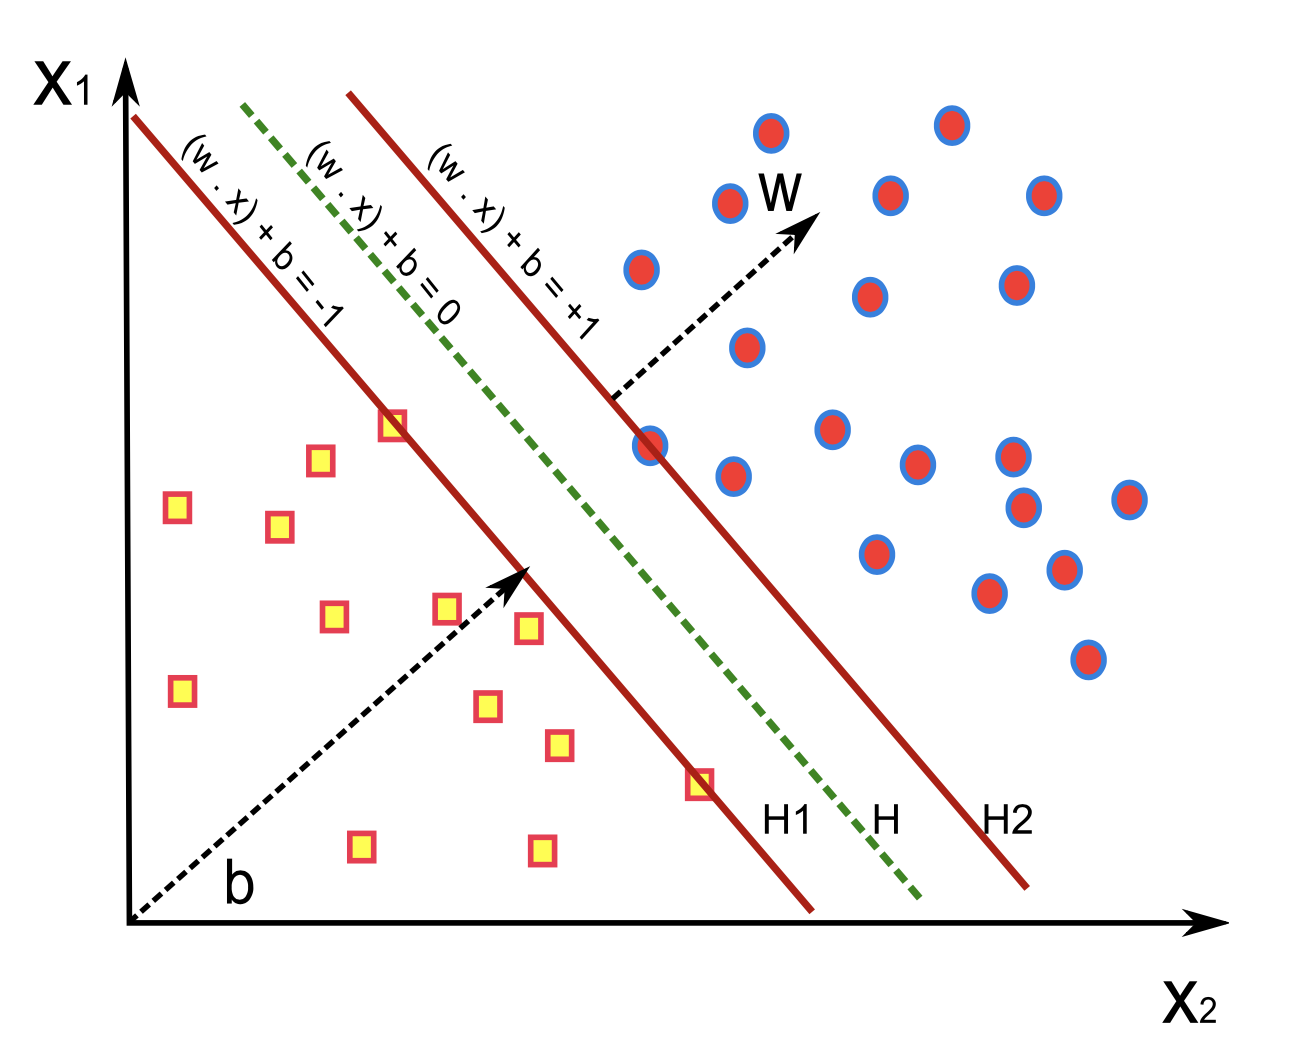
\includegraphics[width=0.6\textwidth]{SVM linearly separable.png}
    \caption{SVM Best Hyperplane in the linearly separable case \cite{cervantesComprehensiveSurveySupport2020}.}
    \label{fig:svm-hyperplane}
\end{figure}

The linearly separable case is rare in real life. Instead, datapoints from one class may seem to mix with the other class at the optimal boundary (Figure \ref{fig:svm-hyperplane-non-linearly-separable}). To still find this optimal boundary, a positive slack factor $\zeta_i$ is introduced and controlled by a parameter $C$ that controls the width of the margin. A lower $C$ allows for a wider margin that may improve generalizability in real life at the cost of more misclassification of the training datatset, whereas a higher $C$ tightens the margin and minimizes the classification errors in the training dataset but may decrease generalizability in real life \cite{cervantesComprehensiveSurveySupport2020}.  

\begin{figure}[ht]
    \centering
    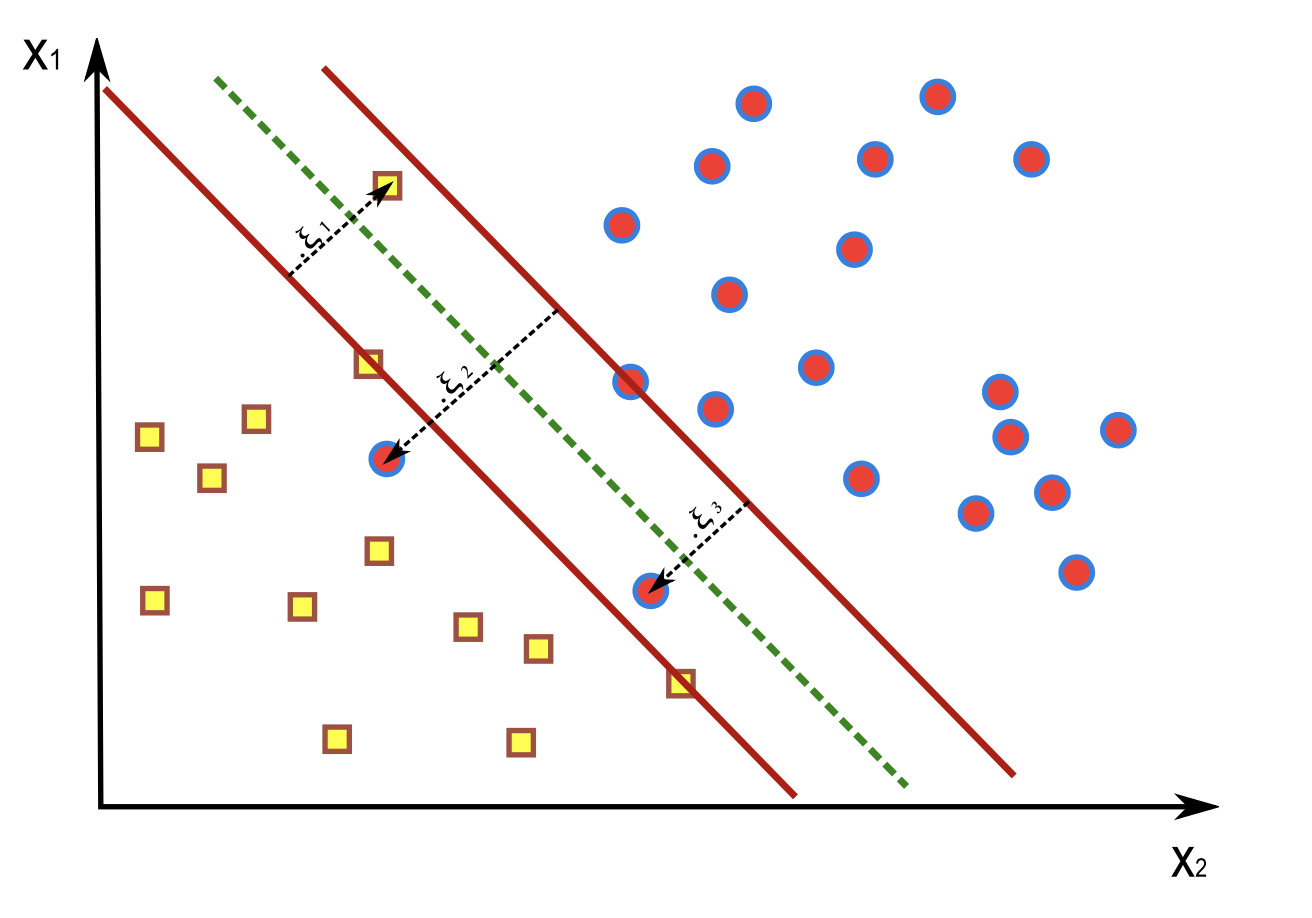
\includegraphics[width=0.6\textwidth]{SVM non-linearly separable.png}
    \caption{SVM Best Hyperplane in the non linearly separable case \cite{cervantesComprehensiveSurveySupport2020}.}
    \label{fig:svm-hyperplane-non-linearly-separable}
\end{figure}

SVM can also be used separate data that is not separable by a linear hyperplane (Figure \ref{fig:svm-hyperplane-non-linearly-classifier}) by using a kernel. Kernels reframe the problem in a highly dimensional space called the "feature space" and in this feature space, it is simple for the algorithm to find the hyperplane. In the next subsection that will detail the convex optimization problem for SVM, it is found that the function that needs to be optimized depends on the inner product between every sample $\langle x_i \cdot x_j \rangle$. Transforming the original dataset to this feature space through a transfer function $\phi$ yields an optimization problem that depends on $\langle \phi(x_i) \cdot \phi(x_j) \rangle$. Kernel functions $K(x_i, x_j)$ are special functions that provide an equivalent way to calculate $\phi(x_i) \cdot \phi(x_j)$ (ie $\phi(x_i) \cdot \phi(x_j) = K(x_i, x_j)$) without having to initially transform the original dataset using $\phi$ since transforming the dataset to the feature space may be a costly operation if there are many features. The following are popular kernels \cite{cervantesComprehensiveSurveySupport2020}:

\begin{enumerate}
    \item Linear Kernel: $K(x_i, x_j) = x_i \cdot x_j$
    \item Polynomial Kernel: $K(x_i, x_j) = (1 + x_i \cdot x_j)^p$
    \item Gaussian Kernel: $K(x_i, x_j) = e^{-\frac{{\left\lVert x_i - x_j\right\rVert}^2}{2\sigma^2}}$
    \item RBF Kernel: $K(x_i, x_j) = e^{-\gamma(x_i - x_j)^2}$
    \item Sigmoid Kernel: $K(x_i, x_j) = tanh(\eta x_i \cdot x_j + v )$
\end{enumerate}

\begin{figure}[ht]
    \centering
    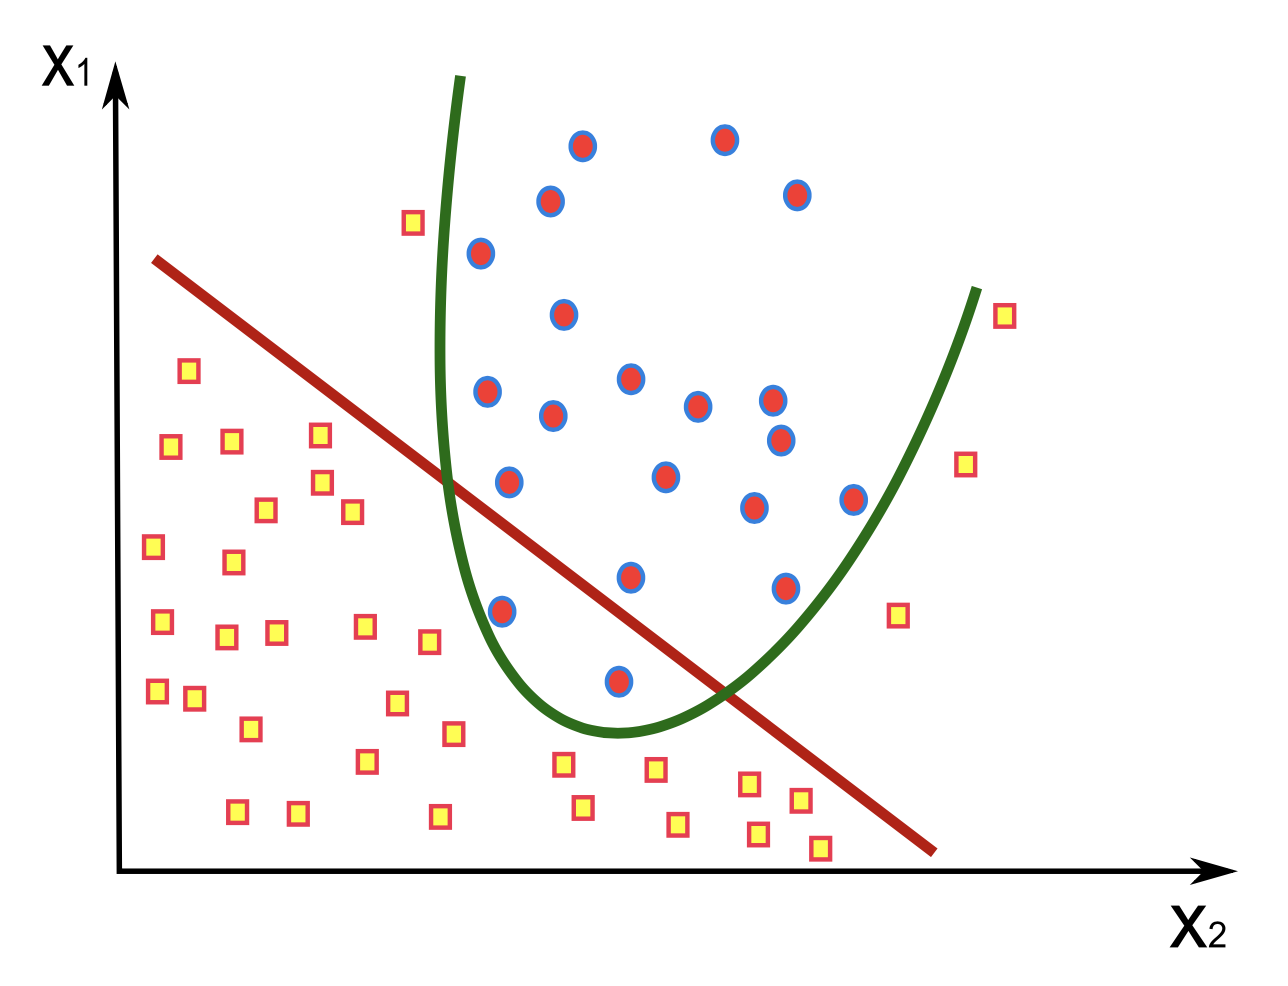
\includegraphics[width=0.6\textwidth]{SVM non-linear classifier.png}
    \caption{SVM non-linear classifier (green line) \cite{cervantesComprehensiveSurveySupport2020}.}
    \label{fig:svm-hyperplane-non-linearly-classifier}
\end{figure}

Since SVM can only separate between 2 classes as a binary classifier, a further step must be done to separate multiple classes. Scikit-learn uses a one vs. rest strategy by default. For each class a decision boundary between itself and the rest of the samples are created. For an unlabeled point a probability of membership to each class is calculated and an argmax function is used to determine the membership \cite{12MulticlassMultioutput}.

\clearpage
\subsubsection{Theory of SVM: Linearly Separable}
Consider a training dataset $X = \{x_i, y_i\}^n_{i=1}$ consisting of $n$ samples of feature vectors $x_i \in \mathbb{R}$ and labels $y_i \in (-1, 1)$. In the linearly separable case of SVM, the two classes in our training dataset can be separated perfectly by a hyperplane. The data labelled with class $y=1$ will be on one side of the hyperplane and the other class $y=-1$ will be on the other side of the hyperplane. The equation for a hyperplane is given in Equation \ref{eq:hyperplane}

\begin{equation}
    \mathbf{w \cdot x} + b = 0
    \label{eq:hyperplane}
\end{equation}

Where $x \in \mathbb{R}^d$, and $\mathbf{w}$ the weights for the hyperplane and $b$ the bias. For simplicity of visualization, consider $x \in \mathbb{R}^2$. The SVM optimization problem tries to find $\mathbf{w}$ and $b$ such that the margin (ie. the distance to the closest point(s) to the hyperplane) is maximized. One variation of this margin called the functional margin $F$ uses the $y_i$ label to ensure that the margin is positive for individual samples correctly classified by some hyperplane with parameters ($\mathbf{w}$, $b$) and is given by the Equation \ref{eq:func_margin}

\begin{equation}
    F = \min_{i=1...n}{[y_i (\mathbf{w} \cdot x_i + b)]}
    \label{eq:func_margin}
\end{equation}

In the SVM optimization problem, this functional margin is set to $F=1$ as shown in \ref{fig:svm-hyperplane} and results in the parallel hyperplanes H1 and H2 as the constraint of the problem (Eq. \ref{eq:svm-constraint}).

\begin{equation}
    y_i (\mathbf{w} \cdot x_i + b) \geq 1 \; \forall \; i
    \label{eq:svm-constraint}
\end{equation}

The goal now is to maximize the distance between the hyperplanes H1 and H2 to obtain the optimal hyperplane H which falls in the middle of H1 and H2. The minimum distance from H to H2 (or H to H1) is called the geometric margin. This minimum distance can be found be taking the vector between any point on H2: $p_{H2}$ and any point on H1: $p_{H1}$ and projecting it onto the unit normal vector of H1 or H2 given by $\mathbf{w}$. Keep in mind that $p_{H2}$ must satisfy $\mathbf{w} \cdot \mathbf{x} + b = 1$ and $p_{H1}$ must satisfy $\mathbf{w} \cdot \mathbf{x} + b = -1$

\begin{equation*}
    \begin{split}
    d &= \left\lVert\text{proj}_\mathbf{w}{(p_{H2} - p_{H1})} \right\rVert \\
     &= \left\lVert \left ((p_{H2} - p_{H1}) \cdot \mathbf{\frac{w}{||w||}}\right ) \frac{\mathbf{w}}{||\mathbf{w}||} \right\rVert \\ 
     &= \left\lVert \left (p_{H2} \cdot \mathbf{w} - p_{H1} \cdot \mathbf{w} \right ) \frac{\mathbf{w}}{||\mathbf{w}||^2} \right\rVert
    \end{split}
\end{equation*}

 $p_{H2}$ must satisfy $\mathbf{w} \cdot p_{H2} + b = 1$ (ie $\mathbf{w} \cdot p_{H2} = b - 1$) to be on hyperplane H2 and $p_{H1}$ must satisfy $\mathbf{w} \cdot p_{H1} + b = -1$ to be on hyperplane H1 (ie $\mathbf{w} \cdot p_{H1} = -b - 1$)

\begin{equation}
    \begin{split}
     &= \left\lVert \left ((1 - b) - (-b - 1) \right ) \frac{\mathbf{w}}{||\mathbf{w}||^2} \right\rVert \\
     &= \left\lVert 2 \frac{\mathbf{w}}{||\mathbf{w}||^2} \right\rVert \\ 
     d &= \frac{2}{||\mathbf{w}||}
    \end{split}
\end{equation}

To find the optimal hyperplane, the distance $d = 2 / ||\mathbf{w}||$ must be maximized or equivalently $||\mathbf{w}||^2$ (which is a convex function \cite{cervantesComprehensiveSurveySupport2020}) can be minimized giving rise to the following convex optimization problem that can be solved using Lagrange Duality. The primal problem is:

\begin{equation}
    \begin{split}
    & \min ||\mathbf{w}||^2 \\
    & \text{s.t.} \; y_i (\mathbf{w} \cdot x_i + b) \geq 1 \; \forall \; i
    \end{split}
    \label{eq:svm-optimization}
\end{equation}

Converting equation \ref{eq:svm-optimization} to the Lagrange Formulation which causes the constraint to move to the objective function and act as a penalty if the constraint is violated:

\begin{equation}
    L(\mathbf{w}, b, \alpha) = \frac{1}{2} \langle \mathbf{w} \cdot \mathbf{w} \rangle - \sum^n_{i=1}{\alpha_i[y_i(\langle \mathbf{w} \cdot x_i \rangle + b) - 1]}
\end{equation}

Setting partial derivatives with respect to $\mathbf{w}$ and $b$ equal to zero to minimize the Lagrangian:

\begin{equation}
    \label{eq:lagrangian-partial-deriv}
    \begin{split}
        \frac{\partial L(\mathbf{w}, b, \alpha)}{\partial \mathbf{w}} = \mathbf{w} - \sum^n_{i=1}{\alpha_i y_i x_i} = 0 & \rightarrow \mathbf{w} = \sum^n_{i=1}{\alpha_i y_i x_i} \\
        \frac{\partial L(\mathbf{w}, b, \alpha)}{\partial b} = - \sum^n_{i=1}{\alpha_i y_i} = 0 & \rightarrow \sum^n_{i=1}{\alpha_i y_i} = 0
    \end{split}
\end{equation}

Substituting these into the Lagrange Formulation and simplifying yields the dual that depends only on the Lagrange Multipliers $\alpha$ \cite{cervantesComprehensiveSurveySupport2020}.

\begin{equation}
    L(\mathbf{w}, b, \alpha) = - \frac{1}{2} \sum_{i=1}^n{\sum_{j=1}^n{\alpha_i y_i \alpha_j y_j \langle x_i \cdot x_j \rangle}} + \sum_{i=1}^n{\alpha_i}
\end{equation}

Then the dual optimization problem is shown in Equation \ref{eq:svm-dual} and the solution to the dual is the same as the solution to the primal given that the Karush-Kuhn-Tucker conditions (KKT) are satisfied \cite{cervantesComprehensiveSurveySupport2020}:

\begin{equation}
    \label{eq:svm-dual}
    \begin{split}
        & \max_{\alpha_i} - \frac{1}{2} \sum_{i=1}^n{\sum_{j=1}^n{\alpha_i y_i \alpha_j y_j \langle x_i \cdot x_j \rangle}} + \sum_{i=1}^n{\alpha_i} \\
        & \text{s.t.} \: \alpha_i \ge 0, \: 1, ..., n \\
        & \: \sum^n_{i=1}{\alpha_i y_i} = 0
    \end{split}
\end{equation}

The solution to the Lagrangian Multipliers $\alpha_i$ can be found using quadratic programming. It is observed that $\alpha_i > 0$ are called the support vectors and all other $\alpha_i = 0$ \cite{cervantesComprehensiveSurveySupport2020}. Once $\alpha_i$ is found, $\mathbf{w}$ can be found using the training data and $\alpha_i$ in Equation \ref{eq:lagrangian-partial-deriv}. Since the support vectors have been found and known to fall on hyperplane H1 and H2, and the normal $\mathbf{w}$ has been found, the optimal $b$ can be found by isolating for $b$ in H2: $(\mathbf{w} \cdot x_{H2}) + b = 1$ or H1: $(\mathbf{w} \cdot x_{H1}) + b = -1$ for a support vector that falls on H2 or H1 respectively.

\subsubsection{Theory of SVM: Not Linearly Separable}\label{sec:not-linearly-separable}
The optimization problem for the not linearly separable case is very similar to the linearly separable case, only now there is the addition of a slack variables $\zeta_i$ to the constraint (see Figure \ref{fig:svm-hyperplane-non-linearly-separable}). The optimization problem then becomes (Equation \ref{eq:soft-margin-opt}) \cite{cervantesComprehensiveSurveySupport2020} with the squared sum of the slack variables modified by a weight $C$ added to the original cost function:

\begin{equation}
    \label{eq:soft-margin-opt}
    \begin{split}
    & \min ||\mathbf{w}||^2 + C \sum_{i=1}^n \zeta_i^2 \\
    & \text{s.t.} \; y_i (\mathbf{w} \cdot x_i + b) \geq 1 - \zeta_i \; \forall \; i \\
    & \:\: \zeta_i \ge 0
    \end{split}
\end{equation}

A higher $C$ increases the cost of permitting slack variables and therefore a higher $C$ tends toward perfectly separating the data. The problem is solved in a similar way using Lagrangian Duality and details can be found in Cervantes et al.'s article \cite{cervantesComprehensiveSurveySupport2020}

\subsubsection{Tunable Parameters}
In SVM the tunable parameters are $C$, the type of kernel selected and the kernel's tunable parameter(s). In Section \ref{sec:not-linearly-separable}, it was discussed that the larger the $C$ the larger the penalty on slack variables and therefore the classifier tends toward perfect separation of the data points. It doesn't seem like there is agreement on what kernel and what kernel parameter is appropriate for a specific application \cite{cervantesComprehensiveSurveySupport2020}. However, in practice it is common for datasets with many features to use the basic linear kernel \cite{cervantesComprehensiveSurveySupport2020}. If the data requires non-linear separation, the Gaussian Kernel is most widely used and its parameter $\sigma$ can be appropriately chosen using a search \cite{cervantesComprehensiveSurveySupport2020}.


\clearpage
\subsection{Random Forests}
\subsubsection{Overview}
Random Forests consist of Decision Trees that must be first discussed \cite{liuNewMachineLearning2012}. A decision tree can be built upon features that are categorical (eg. has astigmatism) or numerical (eg. age). Training a decision tree results in a the structure shown in Figure \ref{fig:decision-tree} with nodes representing the feature and edges representing the options or ranges of values that the feature can take. Typically, the classifier starts at a starting point called the root node. Edges extend uni-directional from the root node presents a decision that the classifier must make based on the features of the new data point. Picking an option or range of values (choosing one of the edges extending from the node) advances the classifier along that edge to the next node in the next level of the tree. The classifier repeats this decision process until there is no more next node; the classifier has reached a "leaf" node and can classify the data point.

\begin{figure}[ht]
    \centering
    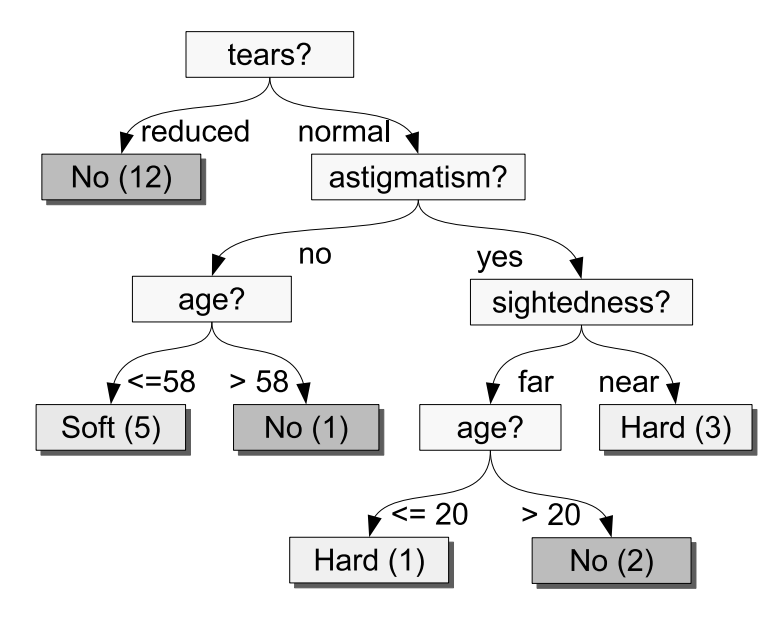
\includegraphics[width=0.6\textwidth]{decision-tree.png}
    \caption{Example of a Decision Tree \cite{leeDecisionTreesTheory}}
    \label{fig:decision-tree}
\end{figure}

Random Forests extend the use of Decision Trees by training multiple trees, classifying the new data with each tree and doing a majority vote on the output of each decision tree \cite{breimanRandomForests2001}. Each Decision Tree is trained using a random subset of data drawn from the original training data with replacement. These trees are grown to maximum depth without pruning using the Classification and Regression Tree (CART) methodology and at each node a random subset of features is used \cite{breimanRandomForests2001}. In situations where there are many features with each feature providing only a small amount of information (eg. medical diagnosis), the single decision tree will have an accuracy slightly better than random classification, whereas using a Random Forest can produce improved accuracy \cite{breimanRandomForests2001}.

In time series data, features can be extracted by taking the mean, standard deviation and slope of random subsequences in sequence labelled a certain class \ref{fig:time-series-rf}. The number of features is then 3 * the number of subsequences extracted. These features are used to train a random forest and new sequences of time series data can be classified by following the same methodology for feature extraction \cite{faouziTimeSeriesClassification2024}.

\begin{figure}[ht]
    \centering
    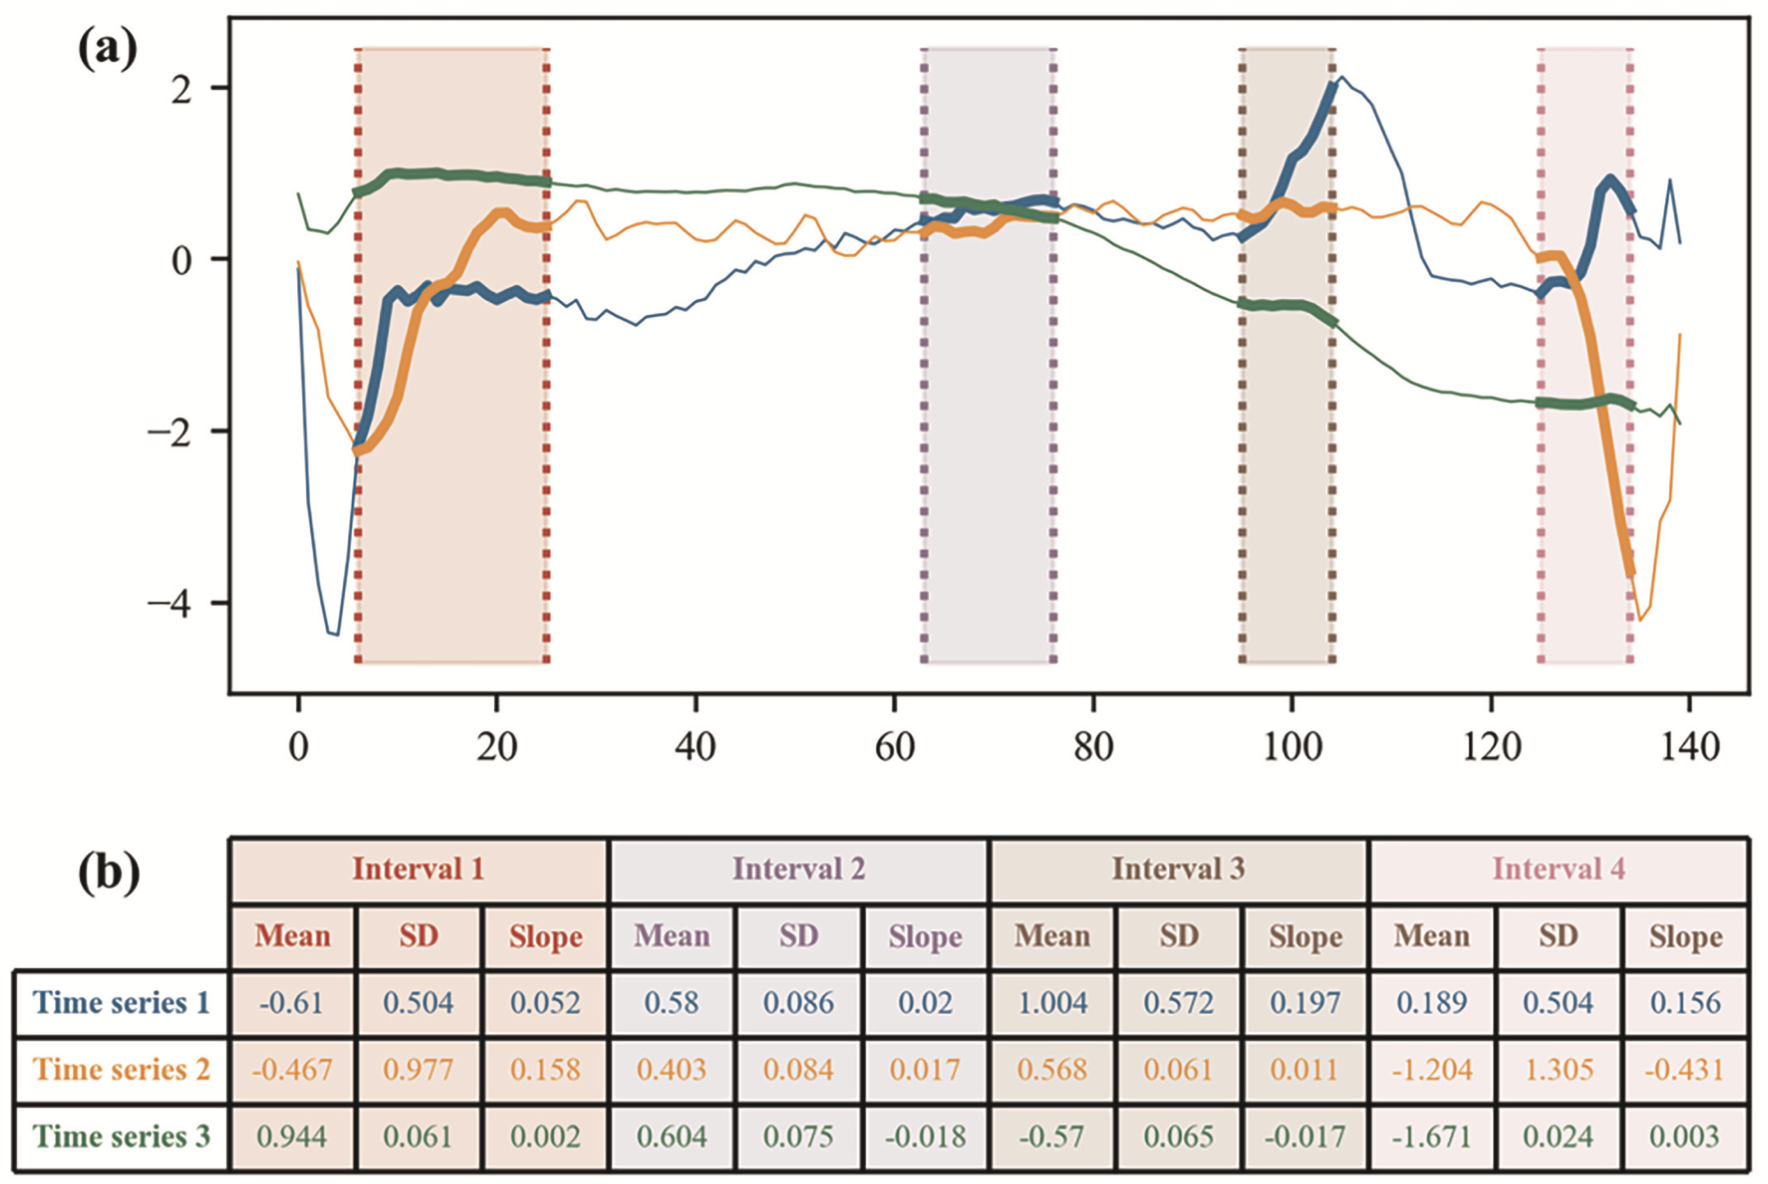
\includegraphics[width=0.8\textwidth]{time-series-random-forest.png}
    \caption{Decision Trees used for time-series classification. Mean, standard deviation and slope of random subsequences in a time-series sequence defining a class are used as features. \cite{faouziTimeSeriesClassification2024}}
    \label{fig:time-series-rf}
\end{figure}


\subsubsection{Classification and Regression Tree (CART) Methodology}
The Classification and Regression Tree (CART) method to grow trees outlined by Breiman et al. has the objectivet of splitting the dataset $L$ at each node such that the descendent nodes--nodes one level down--are "purer" than the parent node. Purity in sklearn's implementation of decision trees can be evaluated using Gini's Impurity and Entropy \cite{10DecisionTrees} and the most common, Gini's Impurity, is shown in Equation \ref{eq:gini} \cite{10DecisionTrees}.

\begin{equation}
    \label{eq:gini}
    \text{G} = \sum_k p_{mk}(1-p_{mk})
\end{equation}

Where $p_{mk}$ is the proportion or probability of observing a class $k$ in subset $Q_m$

\begin{equation}
    p_{mk} = \frac{1}{n_m} \sum_{y \in Q_m}I(y=k)
\end{equation}

At some node $m$, some subset of the data at node $m$ designated as $Q_m$, and $k$ classes. At each node, candidate splits $\theta = (j, t_m)$ consisting of a feature $j$ and threshold $t_m$ are evaluated for impurity. According to the source code for sklearn, these candidate splits are chosen by randomly selecting a feature, sorting the feature's values, and using each of the feature's values as a threshold $t_m$ for a candidate split (ie. the thresholds $t_m$ are the values of feature $j$ for the datapoints in the subset $Q_m$). This process is repeated until the max number of features to be evaluated (an input argument in the Decision Tree Classifier) is reached. The candidate split $\theta$ that minimizes the (Gini) impurity is selected to split the data in a binary fashion with 2 descendant nodes \cite{ScikitlearnSklearnTree}. The same process repeats at the descendent nodes recursively until a termination condition (eg. max depth of tree) is reached or the descendant node only contains a single class.

\subsubsection{Tunable Parameters}
The tunable parameters for Random Forests are similar to Decision Trees and the full list may be found on sklearn's Documentation page for Random Forests \cite{RandomForestClassifier}. Sklearn mentions that the default values for controlling the size of the tree (eg. max\_depth, min\_samples\_leaf) leads to large, unpruned and fully grown trees which may be very memory intensive. They recommend to control these parameters to limit the memory consumption \cite{RandomForestClassifier}. Otherwise, similar to other ML methods, a grid search should be used to find the optimal hyperparameters for the training dataset \cite{probstHyperparametersTuningStrategies2019}. Parameters that should be considered for tuning in order of highest positive effect on the Area Under the Curve (AUC) is mtry (max\_features in sklearn), sample size drawn for training a tree, and the minimum number of observations in a terminal node (min\_samples\_leaf in sklearn) \cite{probstHyperparametersTuningStrategies2019}.

\subsection{Shapelet Transform}

\subsubsection{Overview}
A shapelet is a small but discriminating subsection of a time series waveform that represents a class \cite{yeTimeSeriesShapelets2009}. To classify with shapelets, the authors in \cite{yeTimeSeriesShapelets2009} propose using a decision tree with split criteria based on the inclusion shapelets from a shapelet dictionary (inclusion is determined by the distance between a subsequence from a new time-series signal and the shapelet being less than some threshold--Figure \ref{fig:single-shapelet} shows that the inclusion threshold distance is 5.1). Shapelets address some of the shortcomings of using kNN-DTW presented in Section \ref{sec:knn} that result in large time and space complexity and limit its applicability. 

\begin{figure}[ht]
    \centering
    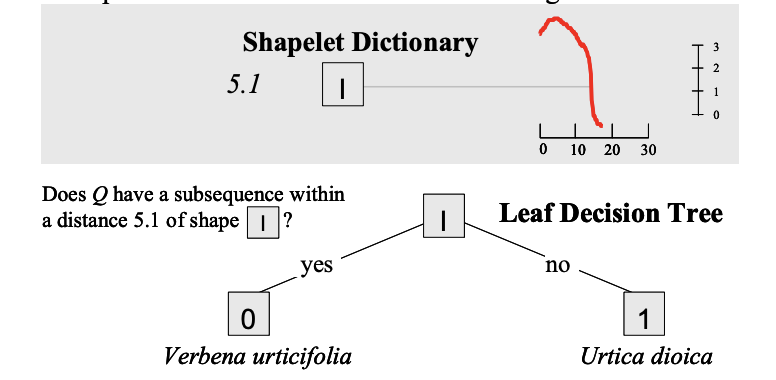
\includegraphics[width=0.6\textwidth]{single-shapelet.png}
    \caption{Example of a shapelet and the criteria for classifying a new time-series \cite{yeTimeSeriesShapelets2009}.}
    \label{fig:single-shapelet}
\end{figure}


\subsubsection{Determining Shapelets}
The authors in \cite{yeTimeSeriesShapelets2009} mention that the total number of possible shapelets can be calculated by the following equation

\begin{equation}
    \sum_{l=MINLEN}^{MAXLEN} \sum_{T_i \in D} (m_i - l + 1)
\end{equation}

for every timeseries $T_i$ in dataset $D$, $l$ is the length of a candidate shapelet and $m_i$ is the length of the $i$-th timeseries in the dataset $D$. For the Trace dataset with has 200 instances, each with length of 275. If $MINLEN=3$ and $MAXLEN=275$, the total number of candidates would be 7,480,200. A brute force approach (Algorithm \ref{alg:shapelet-brute}) would be inefficient at finding the best shapelet. The time complexity is $O(\bar{m}^3k^2)$ for average length of timeseries $\bar{m}$, so the authors propose a pruning strategy to find the best shapelets for classification.

\begin{algorithm}
\caption{Brute Force approach for finding the best shapelet \cite{yeTimeSeriesShapelets2009}, $bsf\_gain$ is the information gain calculated using Entropy.}\label{alg:shapelet-brute}
\begin{algorithmic}
    \State $candidates \gets \text{GenerateCandidates}(D, MAXLEN, MINLEN)$
    \State $bsf\_gain \gets 0$
    \ForEach {$\mathcal{S}$ in $candidates$}
        \State $gain \gets \text{CheckCandidates}(D, \mathcal{S})$
        \If{$gain > bsf\_gain$}
            \State $bsf\_gain \gets gain$
            \State $bsf\_shapelet \gets \mathcal{S}$
        \EndIf
    \EndFor
    \State \Return $bsf\_shapelet$
\end{algorithmic}
\end{algorithm}

To speed up the calculations, the authors use the \textit{early abandon} method in the $\text{CheckCandidates}(D, \mathcal{S})$ function. Instead of calculating the entire Euclidean distance between the shapelet and the subsection of the time series, a minimum distance variable (initialized to infinity) is used to track the minimum distance calculated. If, at any point in the Euclidean distance calculation, the minimum distance is exceeded, the calculation is stopped and moves onto the next step. If the full distance between the shapelet and the subsection of the timeseries is less than the minimum distance in memory, then the minimum distance is updated \cite{yeTimeSeriesShapelets2009}.

Another optimization involves \textit{entropy pruning} which occurs once again at the $\text{CheckCandidates}(D, \mathcal{S})$ function. Another variable is created to store the best so far information gain. Since the minimum distance calculation between the timeseries and the candidate shapelet is the most costly, these distances are calculated one by one. At each distance calculation, the optimal split point is determined for the distances already calculated and the information gain in the most ideal situation (the rest of Class A on one side and the rest of Class B on the other) is calculated. If the information gain in the most ideal situation is less than the best so far gain, then the candidate shapelet can be pruned and no further minimum distance calculations will need to be done. Otherwise, continue calculating the minimum distances between the timeseries and the candidate shapelet and checking the information gain for the ideal situation at each step. If after calculating all of the distances between the candidate shapelet and the the timeseries dataset and the information gain is still greater than the best so far information gain, then the best so far gain is updated and the process continues until all of the candidate shapelets have been considered \cite{yeTimeSeriesShapelets2009}.

\subsubsection{Multi-Class Classification with Shapelets}
To classify multiple classes, the authors of \cite{yeTimeSeriesShapelets2009} proposed growing a decision tree. At each node a shapelet is found using the optimized Algorithm \ref{alg:shapelet-brute} outlined in the previous subsection. The split point identified using the shapelet at the node splits the dataset into a left and right subset of data. On the left and right subset of data, the optimized Algorithm \ref{alg:shapelet-brute} is used to find the shapelet and the split point for that subset of data. The process continues recursively until a leaf node is reached. This process creates a decision tree and a dictionary of shapelets shown in Figure \ref{fig:shapelet-dictionary} that can be used for classifying time-series data.

\begin{figure}[ht]
    \centering
    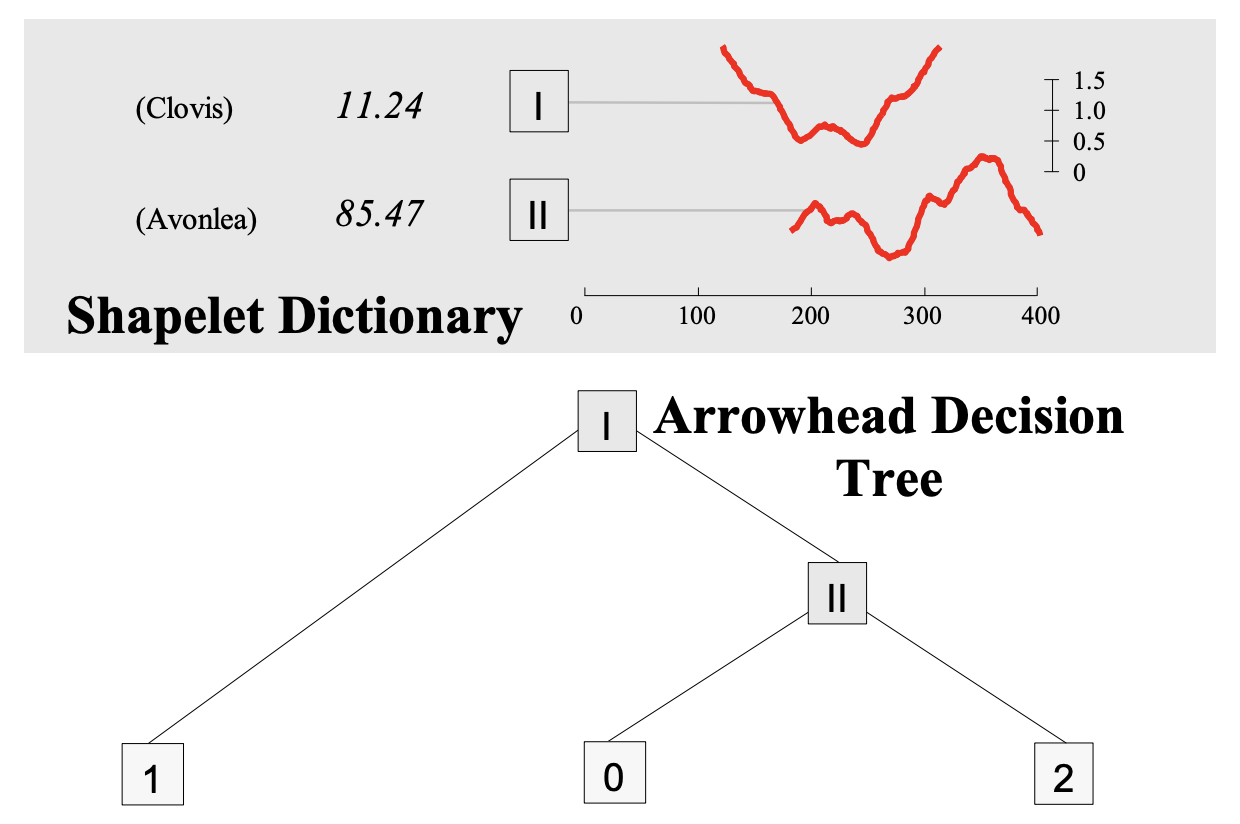
\includegraphics[width=0.6\textwidth]{shapelet-dict.png}
    \caption{An example of a shapelet based decision tree \cite{yeTimeSeriesShapelets2009}.}
    \label{fig:shapelet-dictionary}
\end{figure}

\section{Neural Networks}
\subsection{Overview}
Neural networks are loosely based on the biological structure of the brain; it consists of nodes called neurons which are connected to each other. Some input $x$ passes through the trained layers of neurons and produces an output $f(x,\theta)$ that can be used in applications such as classification (single point output) and forecasting (vector output) \cite{robertsPrinciplesDeepLearning2022b}. An example of a neural network is shown in Figure \ref{fig:neural-net}. Each neuron is a simple function consisting of a weighted sum of the incoming signal added to some bias $b$, and the result $z$ is passed to an activation function $\sigma(z)$ which determines if the neuron \textit{fires} or not. A very simple example of an activation function called the perceptron is shown in Equation \ref{eq:perceptron}. Note that due to the loss of information in the perceptron (ie. no information on the strength of activation), however, it is not used in neural networks found in literature \cite{robertsPrinciplesDeepLearning2022b}.

\begin{figure}[ht]
    \centering
    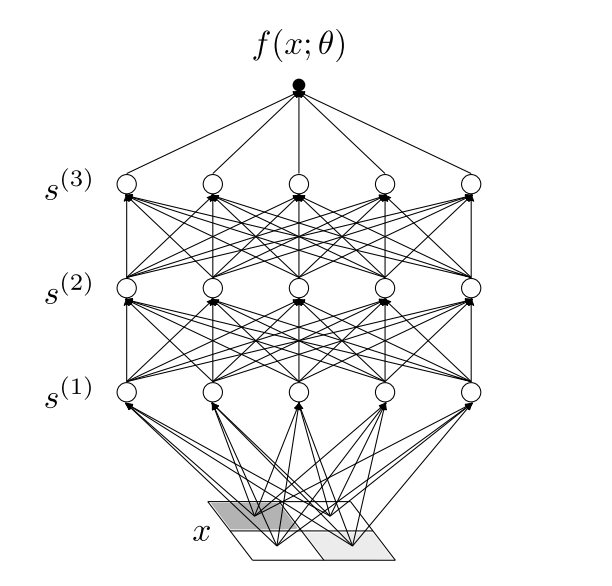
\includegraphics[width=0.6\textwidth]{neural-net.png}
    \caption{A neural network with input $x$ and output $f(x, \theta)$. The input is transformed at each intermediate layer $s^{(1)}, s^{(2)}, s^{(3)}$ until it reaches the output. \cite{robertsPrinciplesDeepLearning2022b}.}
    \label{fig:neural-net}
\end{figure}

\begin{equation}
    \label{eq:perceptron}
    \sigma(z) = \begin{cases} 
        1, & z \geq 0 \\
        0, & z < 1
    \end{cases}
\end{equation}

There are also different types of layers depending on the type of input $x$ and the application of the neural network. The following subsections will briefly discuss these different types of layers used in their respective neural network. These layers include the linear layers, convolutional layers, recurrent layers, long short term memory (LSTM) layers and transformer layers.

\subsection{Deep Neural Networks (DNN)} \label{subsec:DNN}
\subsubsection{The Neuron}
Deep Neural Networks consist of many stacked layers of neurons \cite{robertsPrinciplesDeepLearning2022b}. The threshold for considering a neural network "deep" is 3 layers \cite{WhatNeuralNetwork2021}. As mentioned in the Overview, a neuron consists of the weighted sum of the incoming signal $x$ added to some bias $b$, Equation \ref{eq:neuron}. The weights for each layer are stored in a weight matrix $W$.

\begin{equation}
    \label{eq:neuron}
    z_i(x) = b_i + \sum^{n_{in}}_{j=1}{W_{ij}x_j} \: \text{for} \: i=1,...,n_{out}
\end{equation}

Each $i$-th output goes through an activation function $\sigma_i = \sigma(z_i)$ to determine whether the neuron "fires" to the $i$-th one in the next layer \cite{robertsPrinciplesDeepLearning2022b}. Examples of these activation functions can be seen in Figure \ref{fig:activation-function}. 

\begin{figure}[ht]
    \centering
    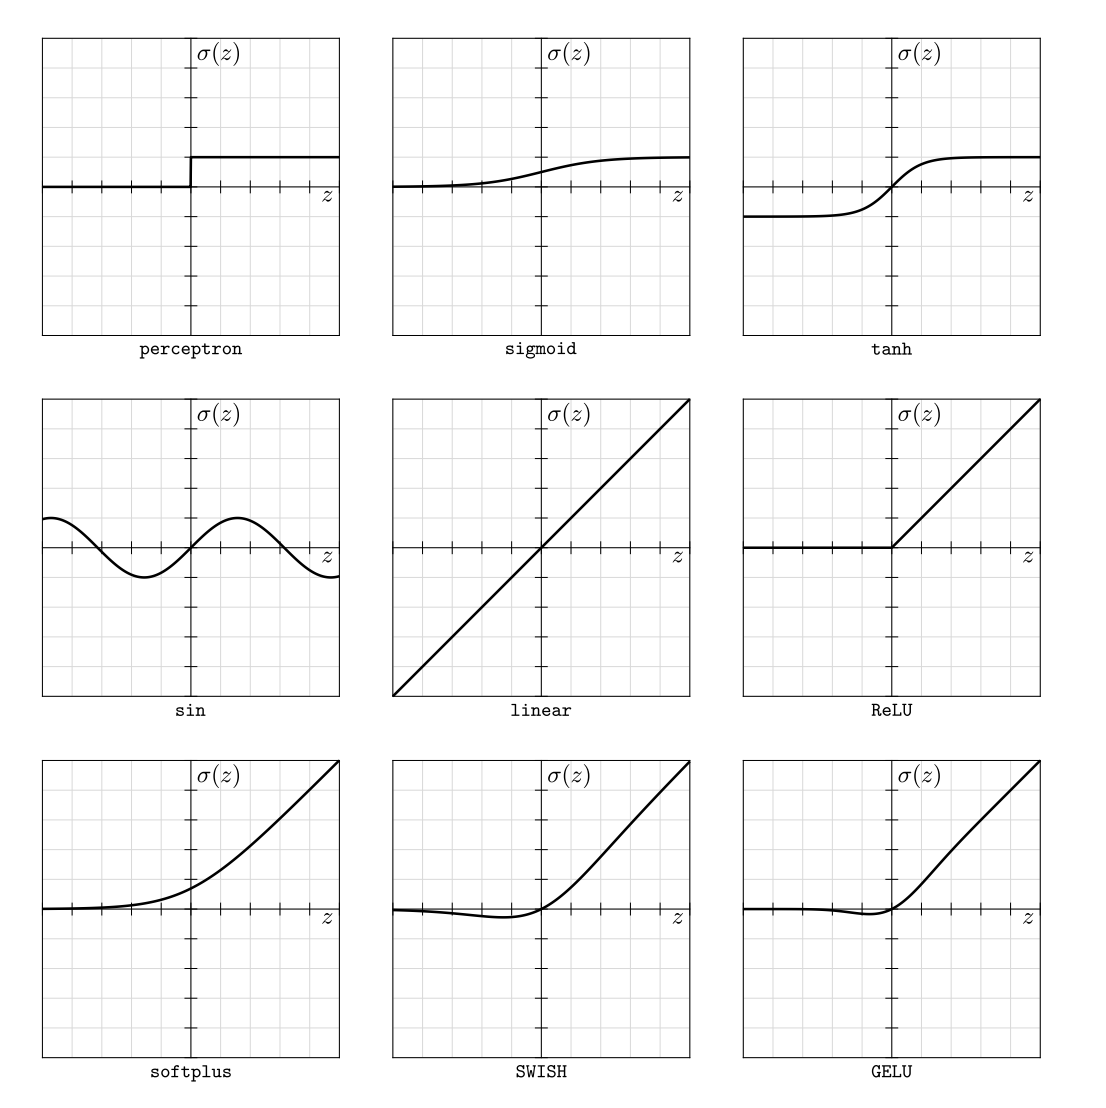
\includegraphics[width=0.8\textwidth]{activation-functions.png}
    \caption{Examples of some activation functions \cite{robertsPrinciplesDeepLearning2022b}.}
    \label{fig:activation-function}
\end{figure}

The inputs and outputs of each layer can then be modeled as follows (Equation \ref{eq:recursive-nn}) with superscripts indicating the layer number \cite{robertsPrinciplesDeepLearning2022b}:

\begin{equation}
    \begin{split}
        \label{eq:recursive-nn}
        z_i^{(1)}(x_\alpha) &= b_i^{(1)} + \sum^{n_{0}}_{j=1}{W_{ij}^{(1)}x_{j;\alpha}} \: \text{for} \: i=1,...,n_{1} \\
        z_i^{(l+1)}(x_\alpha) &= b_i^{(l+1)} + \sum^{n_{l}}_{j=1}{W_{ij}^{(l+1)}\sigma(z_j^{(l)}(x_\alpha))} \: \text{for} \: i=1,...,n_{l+1}, \: l=1,...,L-1
    \end{split}
\end{equation}

Where $L$ is the total number of layers (the depth of the neural network), and $n_{l=1,..,L-1}$ is the number of outputs (the width) at layer $l$. $n_0$ and $n_L$ are the input and output dimensions of the neural network respectively \cite{robertsPrinciplesDeepLearning2022b}. Figure \ref{fig:neural-net-math} depicts the inputs and outputs of a single neuron. 


\begin{figure}[ht]
    \centering
    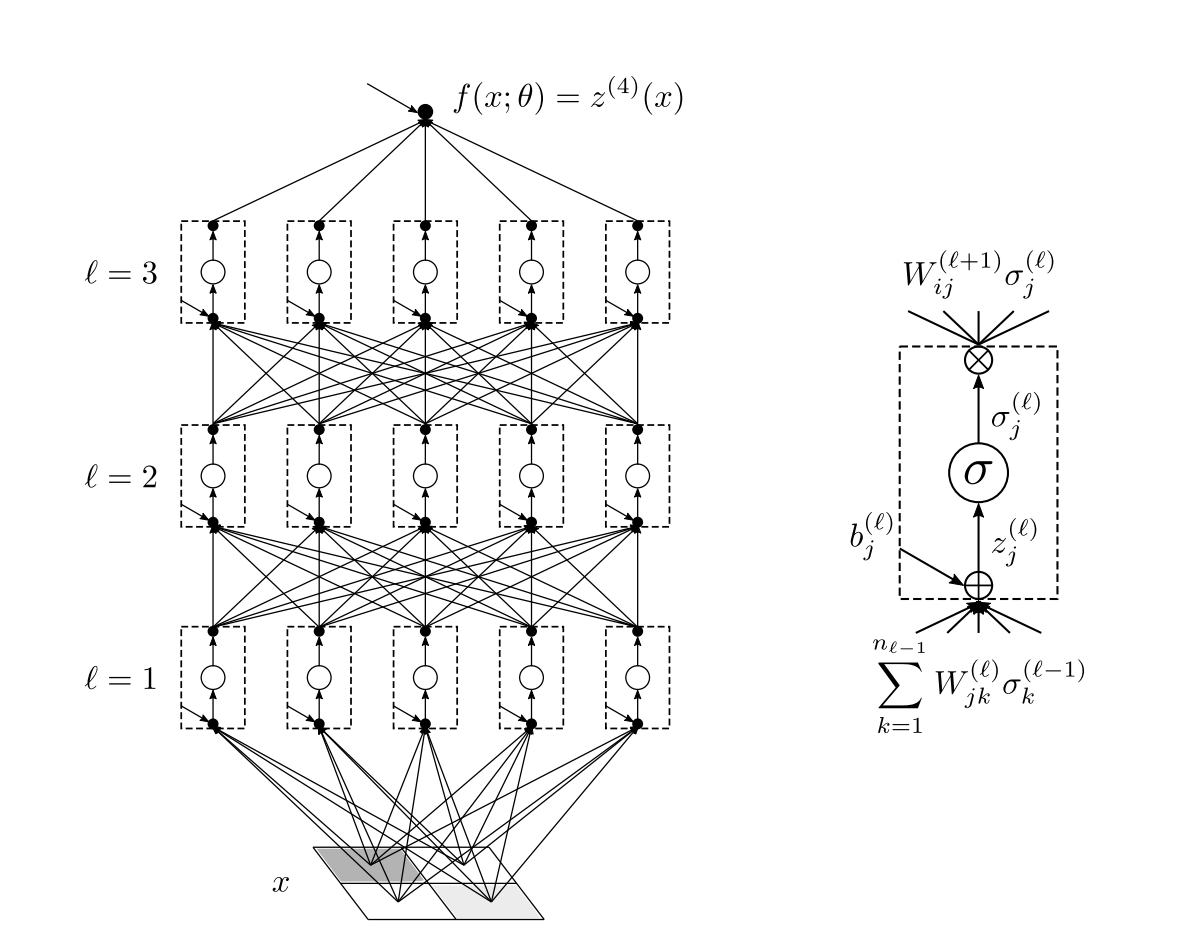
\includegraphics[width=0.9\textwidth]{neural-net-math.png}
    \caption{Visual representation of the equation of a neuron (Equation \ref{eq:recursive-nn}) \cite{robertsPrinciplesDeepLearning2022b}. The image on the right shows the inputs to the neuron and its corresponding outputs.}
    \label{fig:neural-net-math}
\end{figure}

\clearpage
\subsubsection{Training the Neural Network: Gradient Descent}
Training a neural network involves repeatedly updating the weights $W_{ij}$ and biases $b_i$ of the model using a gradient-based method such as gradient descent. Gradient-based methods optimize (minimize) a \textit{loss} function that calculates the error between the output layer result $z^{(L)}(x)$ and the human-annotated labels $y$; the goal of the optimization of the loss function is to decrease the error between the output layer result and the labels. Though the choice of loss function depends on the application, an example of a loss function $\mathcal{L}$ can mean-squared error (MSE) shown in Equation \ref{eq:mse}\footnote{Note that the subscript $\delta$ in $(z(x_\delta;\theta), y_\delta)$ is a placeholder to show the $\delta$-th data point in a certain dataset that $x$ and $y$ are from (ie. training dataset $\mathcal{A}$ has data points $(x_\alpha, y_\alpha)_{\alpha \in \mathcal{A}}$ or testing dataset $\mathcal{B}$ has data points $(x_\beta, y_\beta)_{\beta \in \mathcal{B}}$)} \cite{robertsPrinciplesDeepLearning2022b}.

\begin{equation}
    \label{eq:mse}
    \mathcal{L}_{MSE}(z(x_\delta;\theta), y_\delta) = \frac{1}{2}\left[z(x_\delta; \theta)-y_\delta \right]^2
\end{equation}


With the objective of minimizing the loss in mind, training a simple neural network may have the following steps \cite{robertsPrinciplesDeepLearning2022b}:

\begin{enumerate}
    \item Model parameters $W_{ij}^{(l)}$ and $b_i^{(l)}$ (collectively referred to as $\theta$ hereon) initialized by independently sampling from an easy to sample distribution such as a zero-mean Gaussian Distribution with variances
    \begin{equation}
        \begin{split}
            \mathbb{E}[b_{i_1}^{(l)}b_{i_2}^{(l)}] &= \delta_{i_1 i_2} C_b^{(l)} \\
            \mathbb{E}[W_{i_1 j_1}^{(l)}W_{i_2 j_2}^{(l)}] &= \delta_{i_1 i_2} \delta_{j_1 j_2} \frac{C_W^{(l)}}{n_l - 1}
        \end{split}
    \end{equation}
    With variances $C$ and the above presentation uses the Kronecker Delta $\delta_{i_1 i_2}$ (Equation \ref{eq:kronecker}) to show that the values for each weight and each bias are drawn independently from each other.
    \begin{equation}
        \label{eq:kronecker}
        \delta_{i_1 i_2} = \begin{cases}
            1 & \text{if} \: i_1 = i_2 \\
            0 & \text{if} \: i_1 \neq i_2
        \end{cases}
    \end{equation}

    \item Using the initial weights and biases, the data from the training dataset $\mathcal{A}$ is passed through the neural network using Equation \ref{eq:recursive-nn} which predicts the last layer $z^{(L)}(x_\alpha;\theta)_{\alpha \in \mathcal{A}}$. The loss is then calculated as the average of the loss for each training sample in the training dataset $\mathcal{A}$\ and is shown in Equation \ref{eq:loss}     
    \begin{equation}
        \label{eq:loss}
        \mathcal{L}_{\mathcal{A}}(\theta) \equiv \frac{1}{|\mathcal{A}|} \sum_{\alpha \in \mathcal{A}}\mathcal{L}\left( z^{(L)}(x_\alpha;\theta), y_\alpha \right)
    \end{equation}

    Also note that there can be multiple neurons in the output layer which the label $y_\alpha$ should match in size. The losses from each $i$-th output neuron with the corresponding $i$-th portion of the label for the data point $\alpha$ are summed together. In other words:
    \begin{equation}
        \mathcal{L}_{\mathcal{A}}(\theta) \equiv \frac{1}{|\mathcal{A}|} \sum_{\alpha \in \mathcal{A}} \sum_{i=1}^{n_L} \mathcal{L}\left( z_i^{(L)}(x_\alpha;\theta), y_{i;\alpha} \right)
    \end{equation}


    \item The gradient of this loss is calculated with respect to each model parameter $\theta_\mu$ and is used to iteratively update the model parameters in the negative direction of the gradient\footnote{While Equation \ref{eq:grad-descent} guarantees at least a local minimum with a small learning rate $\eta$. A popular variant of gradient descent called \textbf{Stochastic gradient descent} (SGD) uses a random subset of the training data $\mathcal{S}_t \in \mathcal{A}$. $\mathcal{S}_t$ is called a batch and training is organized into "epochs" which is a complete pass through the training dataset. Using SGD has the advantage of better generalization and scalability since training time scales with a fixed size $\mathcal{S}_t$ instead of the entire training set $\mathcal{A}$ (since Equation \ref{eq:grad-descent} requires the calculation of the gradient for all data points in the data set used, the computation scales linearly with the set used. Assuming that the gradient can be approximated with $\mathcal{S}_t$, computing the gradient with a smaller subset $\mathcal{S}_t$ is faster than the full $\mathcal{A}$ because there are less gradients to calculate).}

    \begin{equation}
        \label{eq:grad-descent}
        \theta_\mu(t+1) = \theta_\mu(t) - \eta \left. {\frac{d\mathcal{L}_\mathcal{A}}{d\theta_\mu}}\right|_{\theta_\mu = \theta_\mu(t)}
    \end{equation}

    Where $\eta$ is a positive hyperparameter called the learning rate and dictates the size of the step in the direction of the negative gradient, $\mu$ is added as a subscript to account for all parameters ($[W_{ij}^{(1)}, b_i^{(1)}, ..., W_{ij}^{(L)}, b_i^{(L)}]$), $t$ is the number of steps in the iterative training process usually starting at $t=0$.

    The derivative $d\mathcal{L}_\mathcal{A} / d\theta_\mu$ is done iteratively starting at the last layer and propagating the results backwards layer by layer. This step is called \textbf{backpropagation} and using the chain rule, it is shown generalized for any parameter $\theta_\mu$ in Equation \ref{eq:gradient_of_param}\footnote{Note that the $dz^{(L)}_{i;\alpha}/d\theta_\mu$ term evaluates to zero if the $i$-th $z_{i;\alpha}^{(L)}$ doesn't depend on the parameter $\theta_\mu$.}:

    \begin{equation}
        \label{eq:gradient_of_param}
        \frac{d\mathcal{L}_\mathcal{A}}{d\theta_\mu} = \sum^{n_{L}}_{i=1} \sum_{\alpha\in\mathcal{A}} \frac{\partial\mathcal{L}_\mathcal{A}}{\partial z_{i;\alpha}^{(L)}} \frac{dz_{i;\alpha}^{(L)}}{d\theta_\mu}
    \end{equation}

     Starting at the last layer $L$ and using the definition of $z_i^{(l+1)}$ in Equation \ref{eq:recursive-nn}, parameters associated with the $m$-th output neuron $m = 1,...,n_L$ can be calculated as\footnote{note that the sum from $i$ to $n_L$ vanishes because $dz_{i;\alpha}^{(L)}/\theta_\mu^{(L)}$ will evaluate to zero if $i \neq m$}:

    \begin{equation}
        \begin{split}
        & \frac{d\mathcal{L}_\mathcal{A}}{d b_m^{(L)}} = \sum^{n_{L}}_{i=1} \sum_{\alpha\in\mathcal{A}} \frac{\partial\mathcal{L}_\mathcal{A}}{\partial z_{i;\alpha}^{(L)}} \frac{dz_{i;\alpha}^{(L)}}{db_m^{(L)}} = \sum_{\alpha\in\mathcal{A}} \frac{\partial \mathcal{L}_\mathcal{A}}{\partial z_{m;\alpha}^{(L)}} (1) \\
        & \frac{d\mathcal{L}_\mathcal{A}}{dW_{mj}^{(L)}} = \sum^{n_{L}}_{i=1} \sum_{\alpha\in\mathcal{A}} \frac{\partial\mathcal{L}_\mathcal{A}}{\partial z_{i;\alpha}^{(L)}} \frac{dz_{i;\alpha}^{(L)}}{dW_{mj}^{(L)}} = \sum_{\alpha\in\mathcal{A}} \frac{\partial\mathcal{L}_\mathcal{A}}{\partial z_{m;\alpha}^{(L)}} \sigma_j^{(L-1)}
        \end{split}
    \end{equation}

    To get the parameters in the subsequent layer $L-1$, the chain rule is once again used:

    \begin{equation}
        \begin{split}
        \frac{d\mathcal{L}_\mathcal{A}}{db_j^{(L-1)}} &= \sum^{n_{L}}_{i=1} \sum_{\alpha\in\mathcal{A}} \frac{\partial \mathcal{L}_\mathcal{A}}{\partial z_{i;\alpha}^{(L)}} \frac{dz_{i;\alpha}^{(L)}}{d\sigma_j^{(L-1)}} \frac{d\sigma_j^{(L-1)}}{dz_{j;\alpha}^{(L-1)}} \frac{dz_{j;\alpha}^{(L-1)}}{db_j^{(L-1)}} \\
        &= \sum^{n_{L}}_{i=1} \sum_{\alpha\in\mathcal{A}} \frac{\partial \mathcal{L}_\mathcal{A}}{\partial z_{i;\alpha}^{(L)}} W_{ij}^{(L)} \sigma_j^{\prime(L-1)} (1) \\
        \frac{d\mathcal{L}_\mathcal{A}}{dW_{jk}^{(L-1)}} &= \sum^{n_{L}}_{i=1} \sum_{\alpha\in\mathcal{A}} \frac{\partial \mathcal{L}_\mathcal{A}}{\partial z_{i;\alpha}^{(L)}} \frac{dz_{i;\alpha}^{(L)}}{d\sigma_j^{(L-1)}} \frac{d\sigma_j^{(L-1)}}{dz_{j;\alpha}^{(L-1)}} \frac{dz_{j;\alpha}^{(L-1)}}{dW_{jk}^{(L-1)}} \\
        &= \sum^{n_{L}}_{i=1} \sum_{\alpha\in\mathcal{A}} \frac{\partial \mathcal{L}_\mathcal{A}}{\partial z_{i;\alpha}^{(L)}} W_{ij}^{(L)} \sigma_j^{\prime(L-1)} \sigma_k^{(L-2)}
        \end{split}
    \end{equation}

    More generally, starting from Equation \ref{eq:gradient_of_param}, the following Equations \ref{eq:backprop-gen} may be used iteratively by sequential multiplication of the chain rule factors to determine the second term in Equation \ref{eq:gradient_of_param} (ie. sensitivity of the output in layer $z_{i;\alpha}^{(L)}$ to parameter $\theta_\mu$: $dz_{i;\alpha}^{(L)}/d\theta_\mu$) in the $l$-th layer $l=L-1,...,1$ (once again working backwards from layer $L$):

    \begin{equation}
        \label{eq:backprop-gen}
        \begin{split}
        \frac{dz_{i;\alpha}^{(L)}}{db_j^{(l)}} &= \frac{dz_{i;\alpha}^{(L)}}{dz_{j;\alpha}^{(l)}} \\
        \frac{dz_{i;\alpha}^{(L)}}{dW_{jk}^{(l)}} &= \sum_m \frac{dz_{i;\alpha}^{(L)}}{dz_{m;\alpha}^{(l)}} \frac{dz_{m;\alpha}^{(L)}}{dW_{jk}^{(l)}} = \frac{dz_{i;\alpha}^{(L)}}{dz_{j;\alpha}^{(l)}}\sigma_{k;\alpha}^{(l-1)} \\
        \frac{dz_{i;\alpha}^{(L)}}{dz_{j;\alpha}^{(l)}} &= \sum^{n_{l+1}}_{k=1} \frac{dz_{i;\alpha}^{(L)}}{dz_{k;\alpha}^{(l+1)}}W_{kj}^{(l+1)}\sigma_{j;\alpha}^{\prime (l)} \quad \text{for} \quad l<L
        \end{split}
    \end{equation}

    As a rule of thumb, The change in the loss function $\mathcal{L}_{\mathcal{A}}$ with respect to some parameter $\theta_\mu^{(l)}$ in layer $l < L$ will depend on all of the neurons in the layer above $l+1$ (causing the summations to stack as the change in the loss function with parameters in lower layers are calculated).

    Equation \ref{eq:grad-descent} is run until there is convergence at a least a local minimum or the number of iterations specified is completed \cite{robertsPrinciplesDeepLearning2022b}.
\end{enumerate}

After the model parameters have been trained, the forward equation (Equation \ref{eq:recursive-nn}) can be used on new input data to classify, predict or forecast whatever the model was trained to do.


\clearpage
\subsection{Convolutional Neural Networks (CNN)}
Convolutional Neural Networks (CNN) are typically used for inputs that are in the shape of a 2D arrays with multiple channels (ie. the depth of the input) such as a color image with RBG channels. They are primarily used in image recognition and classification tasks \cite{tayeTheoreticalUnderstandingConvolutional2023}. Unlike the DNN in Section \ref{subsec:DNN} which requires a set of features to input into the model, CNNs extract the features from images by themselves during the training and do not require the user to determine a set of features. Typically, CNNs are composed of 3 layers \cite{tayeTheoreticalUnderstandingConvolutional2023,prakashAdvancedDeepLearning2021}: 

\begin{itemize}
    \item Convolutional
    \item Pooling
    \item Fully Connected (discussed in \ref{subsec:DNN})
\end{itemize}

A typical architecture for a CNN is outlined in Figure \ref{fig:cnn-architecture}. 

\begin{figure}[ht]
    \centering
    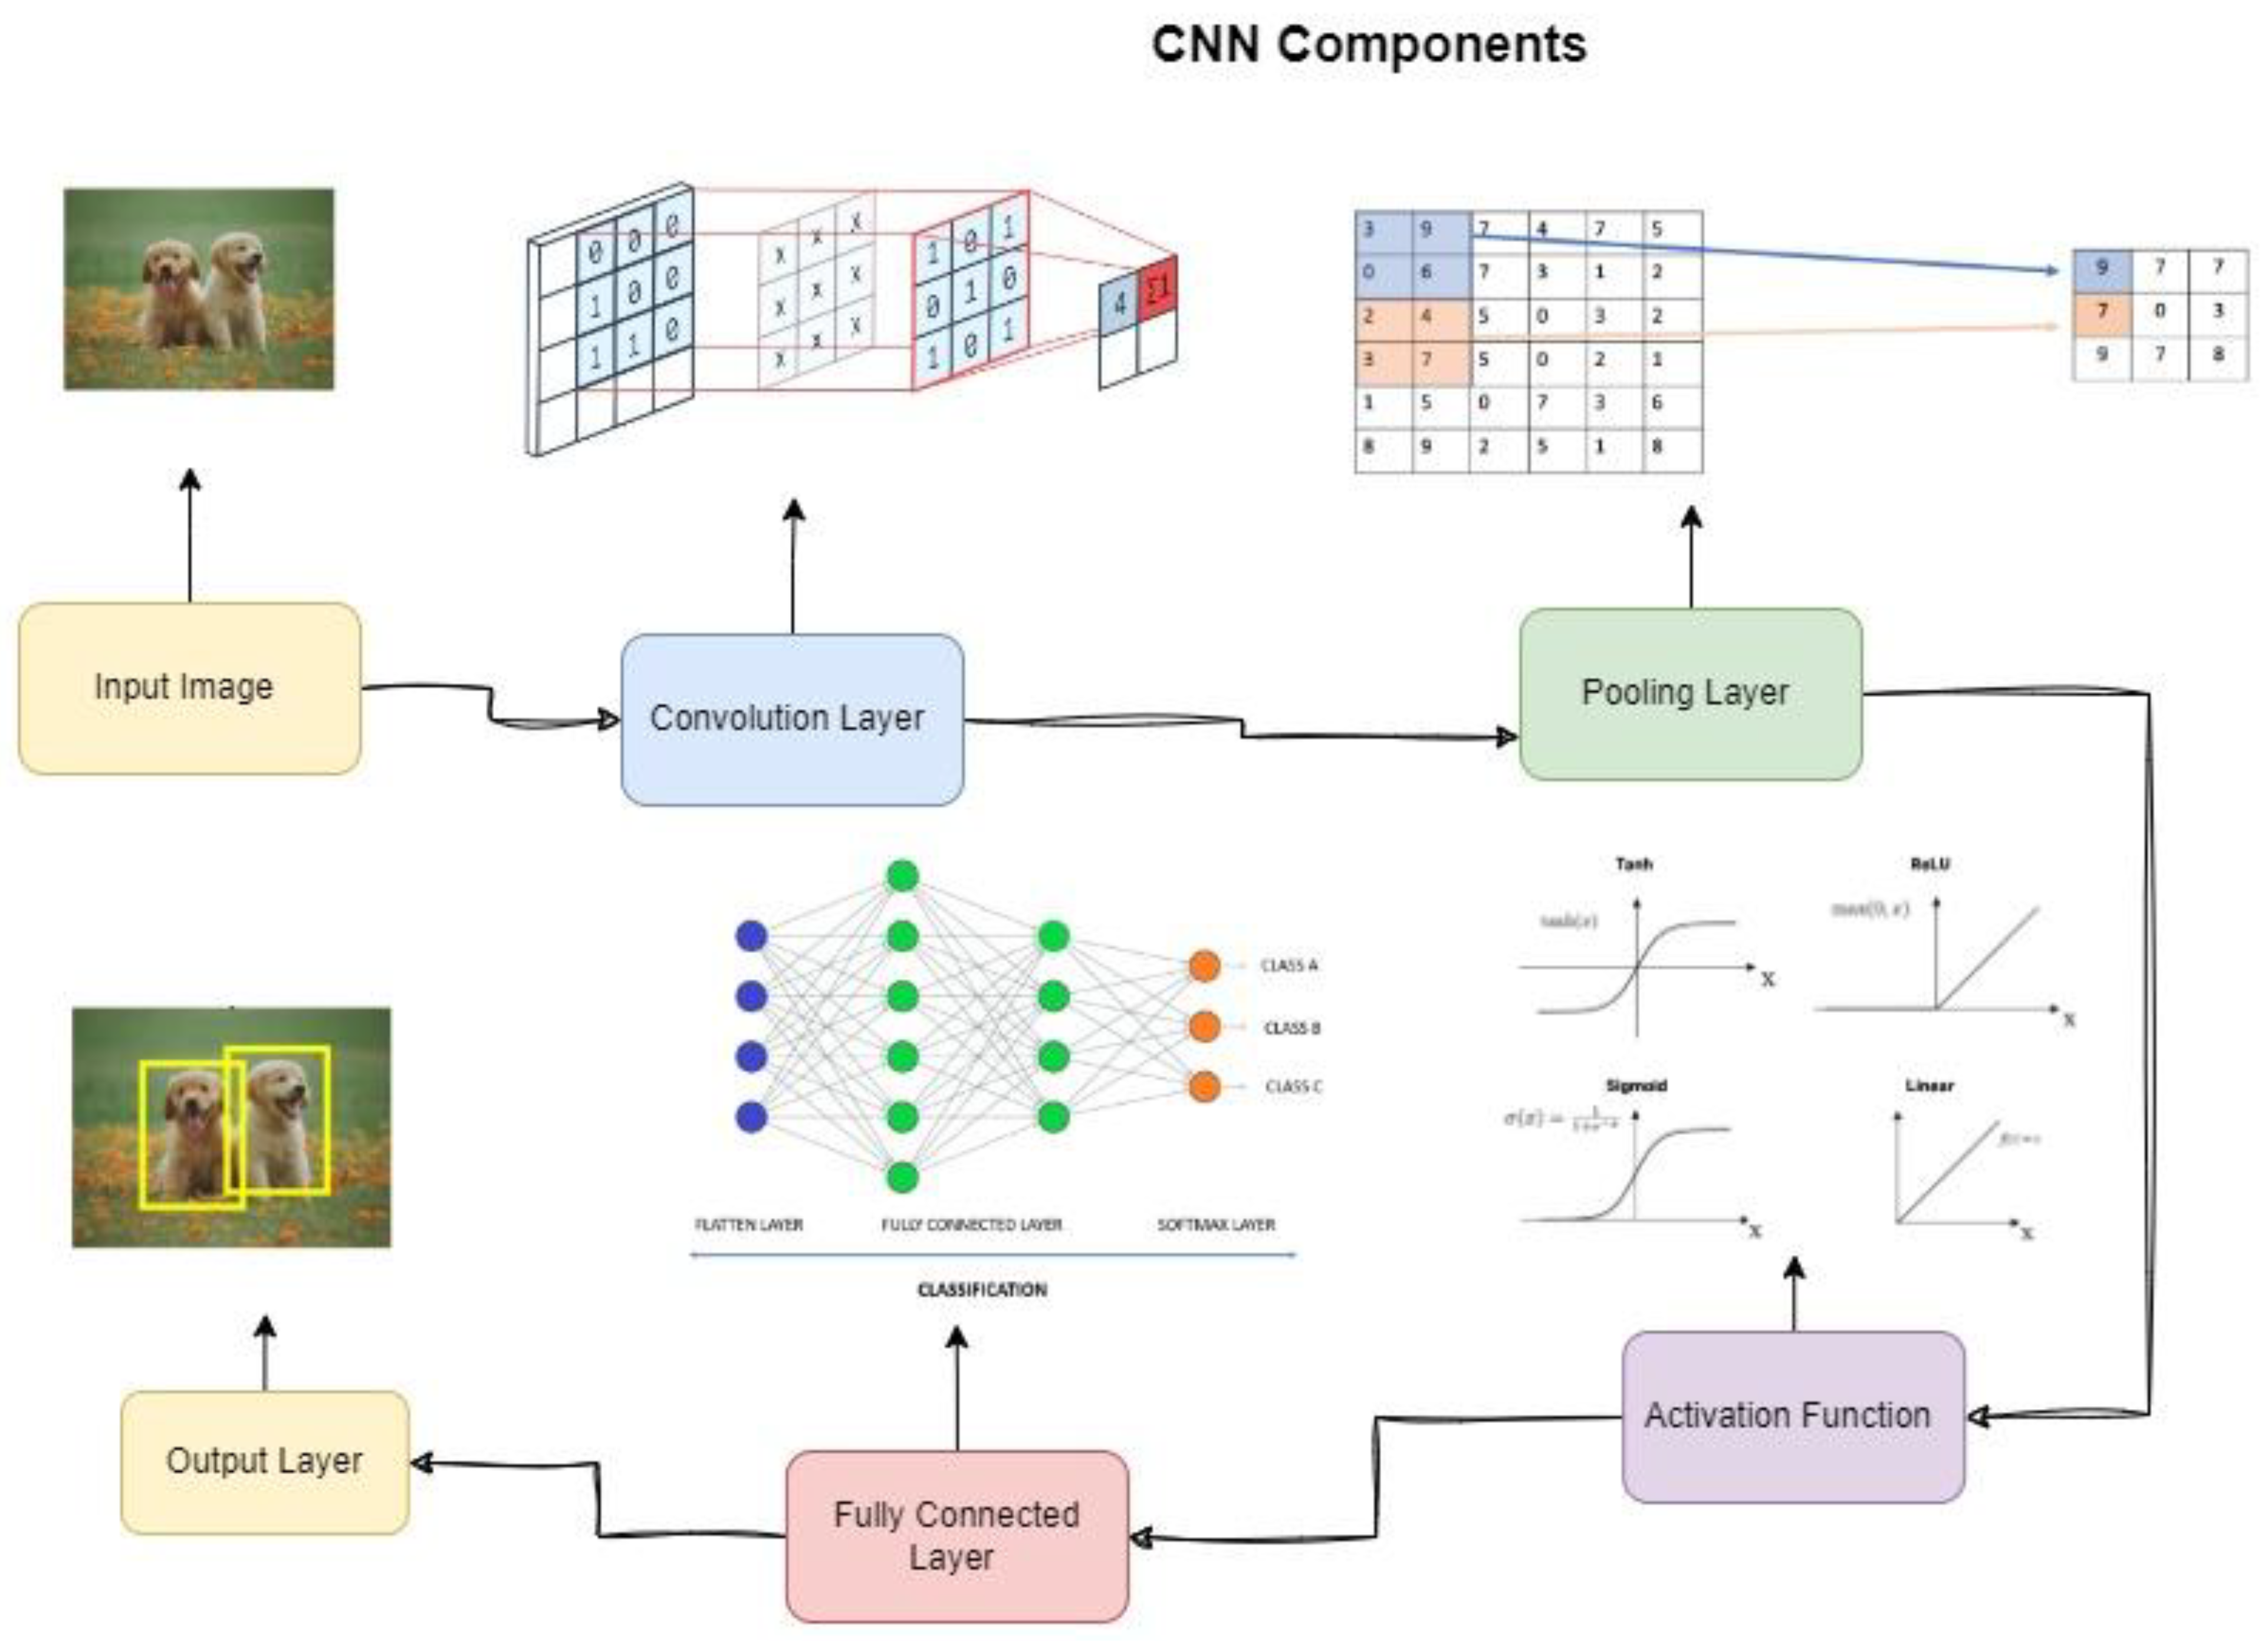
\includegraphics[width=0.8\textwidth]{cnn.png}
    \caption{Architecture of a common CNN \cite{tayeTheoreticalUnderstandingConvolutional2023}.}
    \label{fig:cnn-architecture}
\end{figure}

\subsubsection{Convolutional Layer}
The convolutional layer involves applying a set of \textbf{filters} or \textbf{kernels} to the data before it is used (the user can specify the number of kernels $k$ in each layer). These kernels are small 3D arrays whose height and width $F$ are typically smaller than the input array's but have the same depth $r$ as the input array. The kernel's values are called \textbf{weights} and are trainable. 

Initially, the weights are initialized at random, but as the training progresses, the weights change to enable the kernel to extract meaningful features \cite{tayeTheoreticalUnderstandingConvolutional2023}. In the forward pass, the kernel transforms the image through the dot product between the kernel and the section of the input array. The kernel starts at the top left of the input array and slides left to right, top to bottom calculating the dot product between itself and the section of the input array to produce a single value at each step. How much the filter slides is controlled by the \textbf{stride} parameter (ie. a stride of 1 means that the filter will slide to the right 1 element every step where as a stride of 2 means that the filter will stride to the right 2 elements every step). Figure \ref{fig:cnn-filters} shows the result of applying a 2x2 kernel on a 4x4 input with a stride of 1.

\begin{figure}[ht]
    \centering
    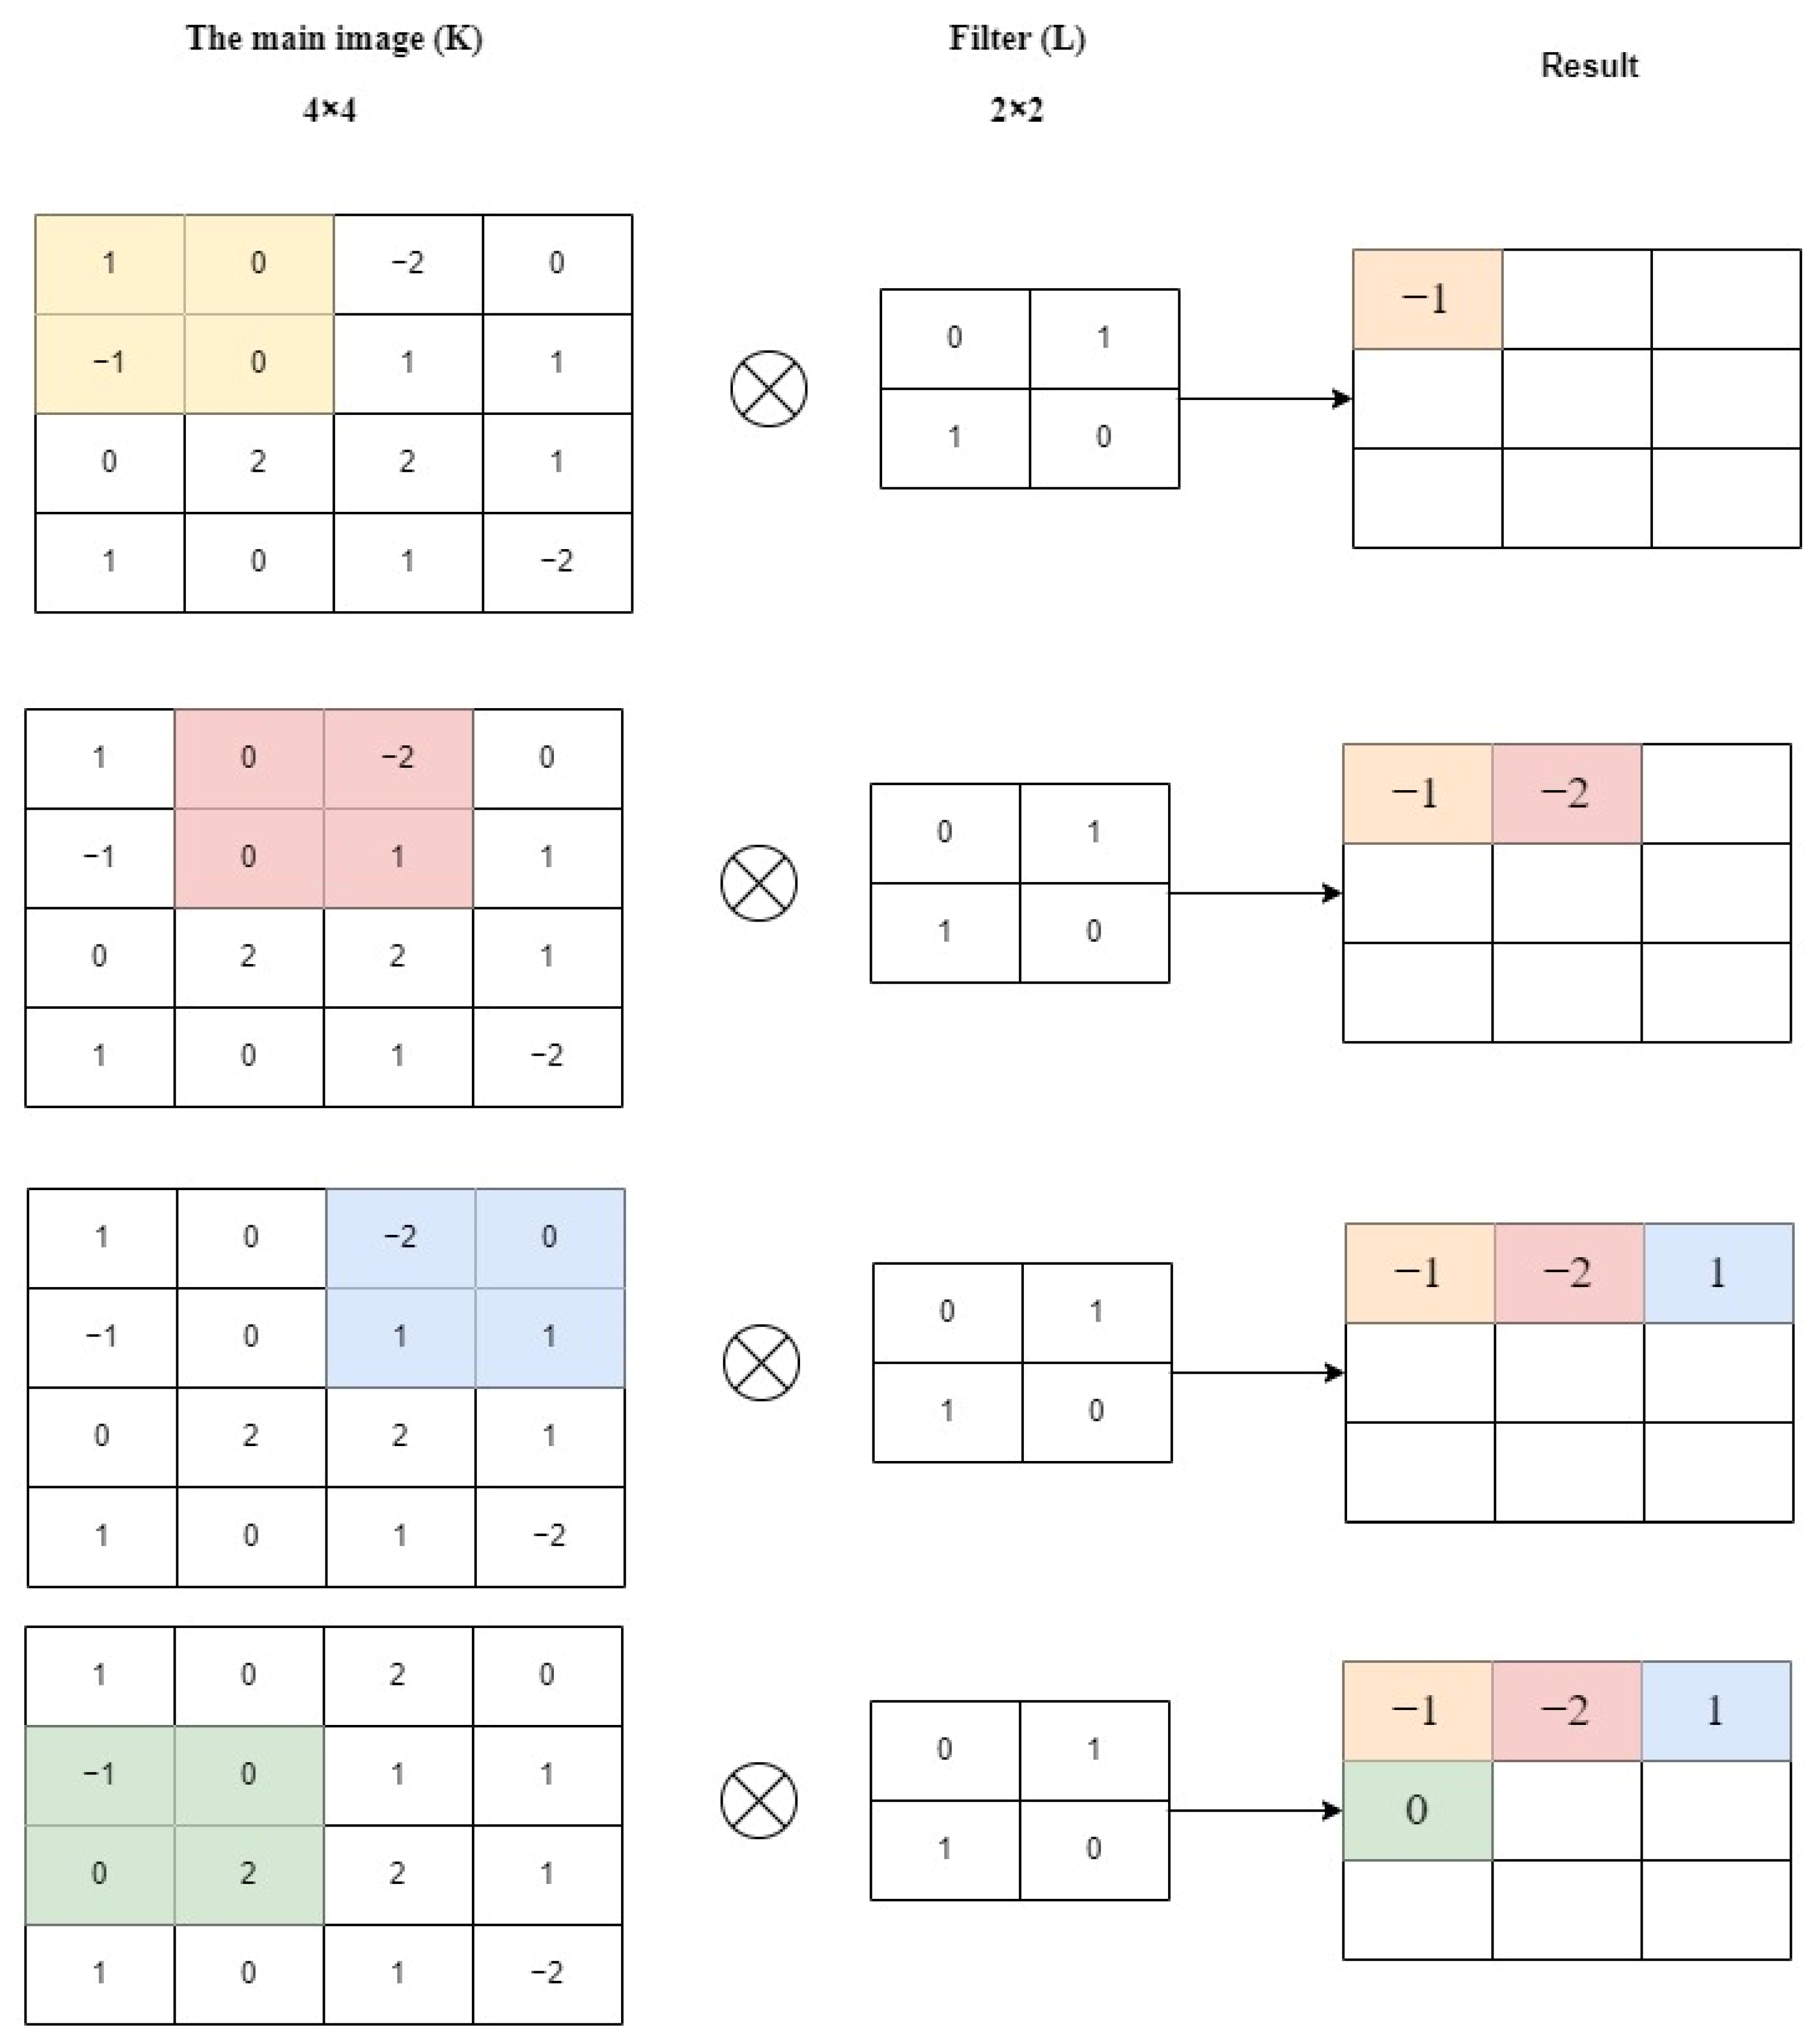
\includegraphics[width=0.8\textwidth]{cnn-filters.png}
    \caption{Applying a kernel (filter) to the input array \cite{tayeTheoreticalUnderstandingConvolutional2023}.}
    \label{fig:cnn-filters}
\end{figure}



As seen in Figure \ref{fig:cnn-filters} the output height and width was less than the input array's height and width. To avoid the shrinkage in size after applying the kernel, the input array can be zero padded $P$ number of layers. Taye's \cite{tayeTheoreticalUnderstandingConvolutional2023} formula to calculate the expected output dimension's height and width $O$ after applying a kernel with height and width $F$, input array height and width $N$, and stride $S$ is shown in Equation \ref{eq:cnn-out-dim}

\begin{equation}
    \label{eq:cnn-out-dim}
    O = 1 + \frac{N + 2P - F}{S}
\end{equation}

The convolutional operation from one kernel will produce an array with shape ($O$,$O$,1). For $k$ number of kernels that the user defines, the final output shape will be ($O$,$O$,$k$).

After the convolution operation is complete, a bias $b$ is added to the output from each kernel and the values are typically passed through the ReLU activation function $\sigma$ to remove the negative values\footnote{though a Leaky ReLU may be used to avoid the "Dying ReLU" issue} \cite{tayeTheoreticalUnderstandingConvolutional2023,purwonoUnderstandingConvolutionalNeural2023}. In other words, the output $z^{k, (l)}$ at layer $l$ for the $k$-th kernel (that is passed to the next layer) is as follows for some input $x$ \cite{alzubaidiReviewDeepLearning2021}:

\begin{equation}
   \label{eq:cnn-output}
    z^{k, (l)} = \sigma(W^{k, (l)} * x + b^k)
\end{equation}


Where $W^{k, (l)}$ are the weights of the $k$-th kernel, $b^k$ is the bias added to the output of the $k$-th kernel, and the $*$ symbol represents the convolution operation.

Based on the information discussed on convolutions, given kernel height and width\footnote{height and width of the kernel do not always need to be the same.} $F$, the number of filters $k$ and the depth of the input layer $r$, the number of trainable parameters in one convolutional layer is shown in Equation \ref{eq:cnn-num-params}

\begin{equation}
    \label{eq:cnn-num-params}
    \text{Number of Parameters} = ((F * F * r) + 1)k
\end{equation}

\subsubsection{Pooling Layer}
Pooling downsamples the output to decrease the height and width dimensionality while retaining the most important data. Similar to the idea of a filter or kernel in the previous section, the pooling filter can have the height and width specified (eg. 2x2) as well as the type (eg. max, min, avg). The pooling filter starts at the top left and slides left to right, top to bottom applying the pooling rule to section of the input to the pooling filter. For example, if the pooling type is a max, the maximum value in the section of the input array where the pooling filter is at is taken and becomes the new value in the shrunken output array. Typically, the pooling filter then slides with a stride equal to its dimensions: $S=F$. The pooling layer operates over all of the channels such that the height and width are reduced, but the depth remains the same \cite{tayeTheoreticalUnderstandingConvolutional2023}. Taye provides an example of Max Pooling and Average Pooling with a 2x2 filter size in Figure \ref{fig:cnn-pooling}. Similar to the convolutional layer, the output height and width $O$ can be calculated using Equation \ref{eq:cnn-out-dim} with no padding (ie. $P=0$) and the depth of the output is the same as the input. 

\subsubsection{Fully Connected Layer}
In CNN architectures such as AlexNet and LeNet-5 \cite{swapnaCNNArchitecturesAlex2020} and the sample CNN architecture in pyTorch \cite{TrainingClassifierPyTorch} the output from the last pooling layer is flattened into a 1D array and fed as an input to fully connected layers discussed in Section \ref{subsec:DNN}. From the literature, it seems that the ReLU activation function is the most popular for its simplicity and time and resource savings \cite{tayeTheoreticalUnderstandingConvolutional2023,swapnaCNNArchitecturesAlex2020,prakashAdvancedDeepLearning2021}.

\begin{figure}[ht]
    \centering
    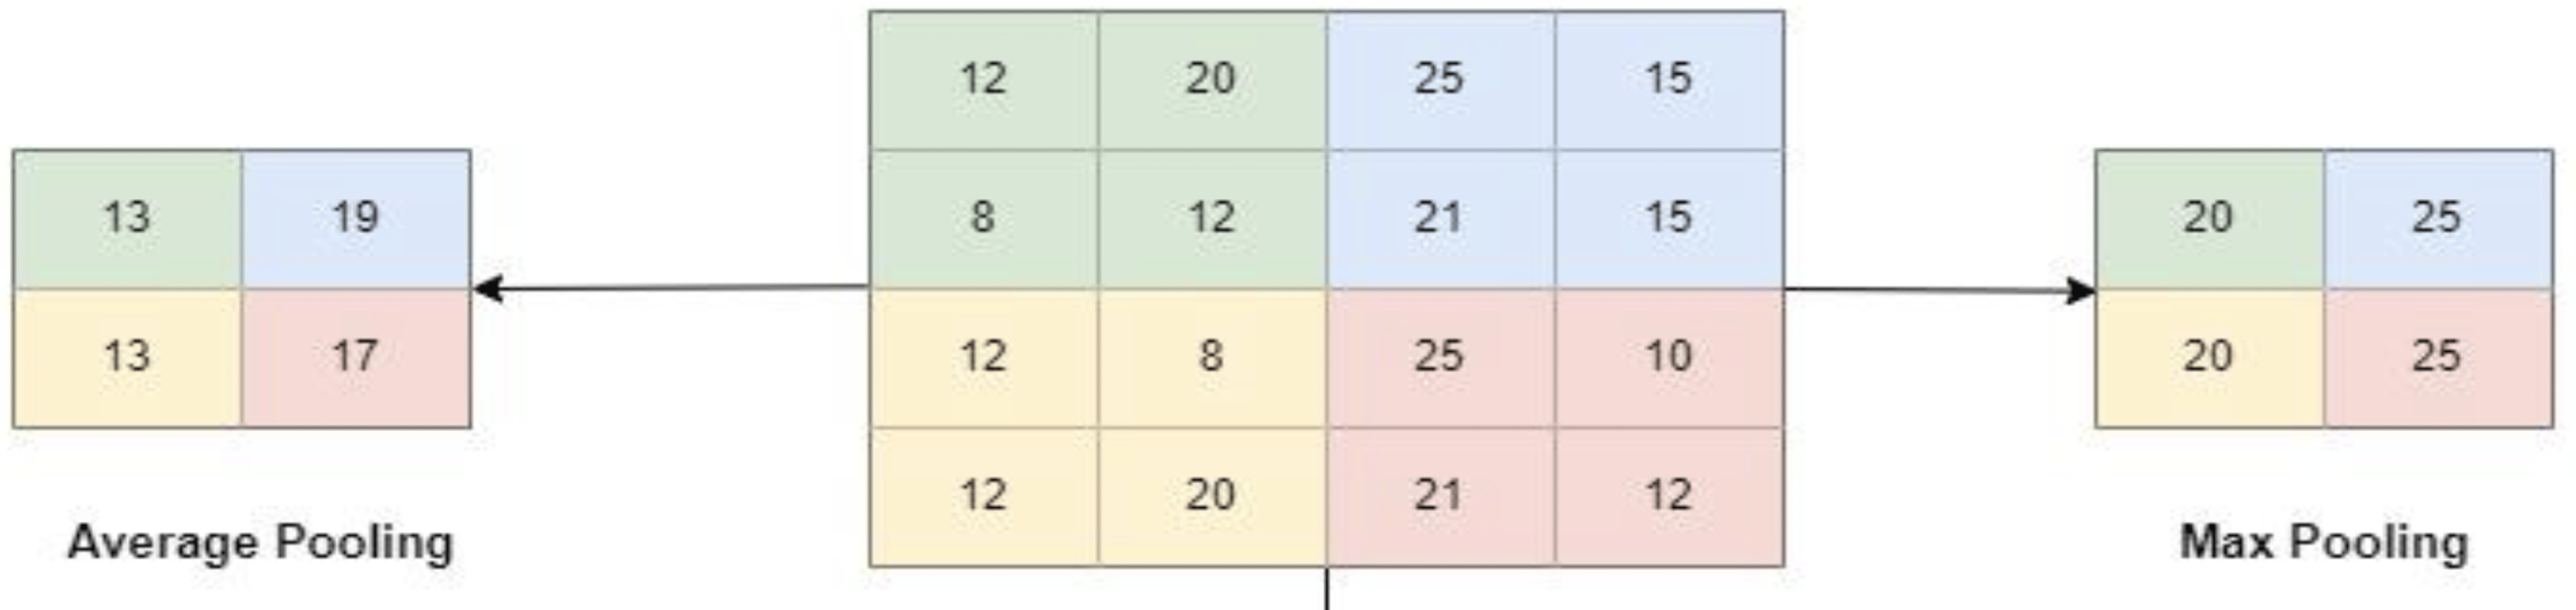
\includegraphics[width=0.9\textwidth]{pooling.png}
    \caption{The pooling layer \cite{tayeTheoreticalUnderstandingConvolutional2023}}
    \label{fig:cnn-pooling}
\end{figure}

\subsubsection{Training the Convolutional Layers}
Similar to the training done in the DNN section, training the convolutional layers involve backpropagation and finding the gradient of the cost function with respect to all of the model's parameters. Then using gradient descent, the optimal parameters may be found. Recall Equation \ref{eq:grad-descent}:

\begin{equation}
    \theta_\mu(t+1) = \theta_\mu(t) - \eta \left. {\frac{d\mathcal{L}_\mathcal{A}}{d\theta_\mu}}\right|_{\theta_\mu = \theta_\mu(t)}
\end{equation} 

First backpropagation is done through the fully connected layers to find the $d\mathcal{L}_\mathcal{A}/d\theta_\mu$ for weights and biases in the fully connected layers. This has already been discussed in Section \ref{subsec:DNN} through the use of the chain rule. Considering that a typical CNN architecture involves stacking of the Convolutional layers and the Pooling layers prior to the fully connected layers (refer to Figure \ref{fig:alexnet} of AlexNet), calculating the weights and biases that are in the Convolutional layers requires backpropagation to work backwards through both the pooling and the convolutional layers. The treatment of the pooling and convolutional layers will be discussed next.

\begin{figure}[ht]
    \centering
    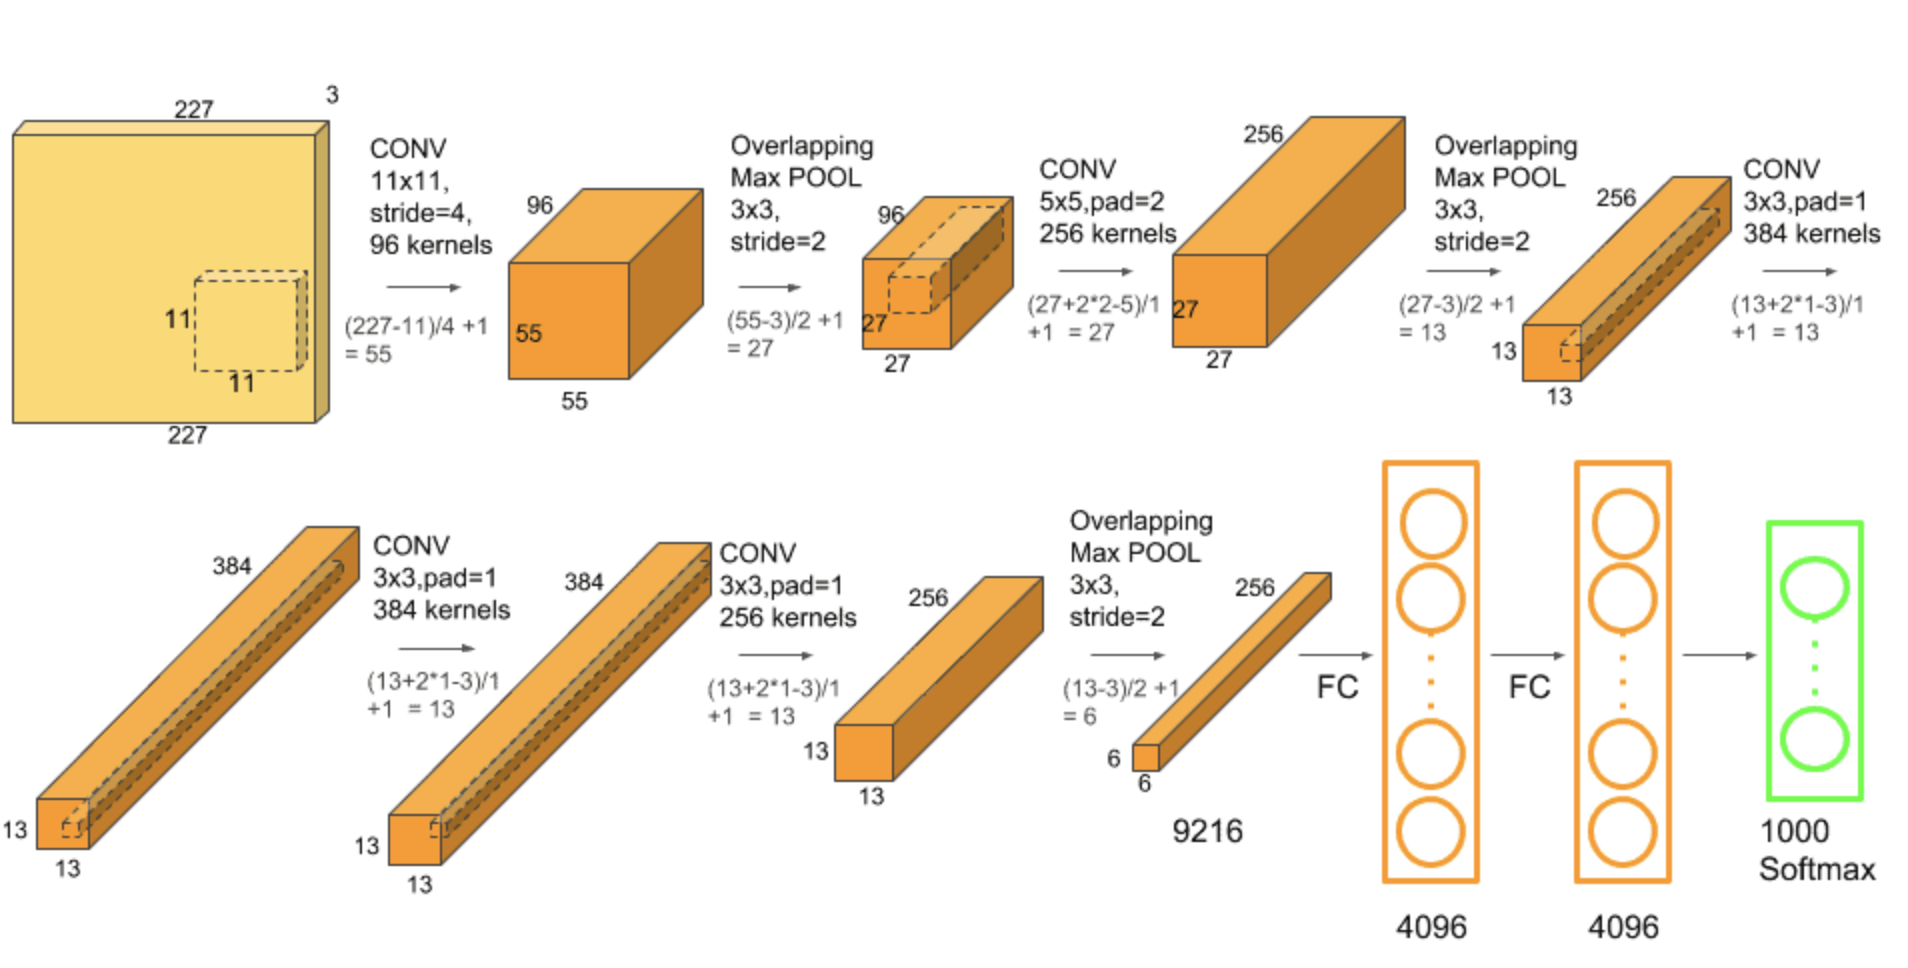
\includegraphics[width=0.9\textwidth]{alexnet.png}
    \caption{Architecture of the AlexNet \cite{vasudevUnderstandingCalculatingNumber2020}.}
    \label{fig:alexnet}
\end{figure}


Since there are no parameters in the pooling layer, we must look back to the convolutional layer prior to this pooling layer to see how the pooling layer affects the backpropagation. Each cell $z_{ij}^{k, (l)}$ in the output from the convolutional layer is dependent on all the weights in the $k$-th kernel. Using $ij$ subscripts to denote the position in the output 2D array, $k$ to denote the $k$-th kernel, $F$ as the width and height of the kernel, $r$ the depth of the kernel and $O$ the output height and width, Equation \ref{eq:cnn-output} expanded is shown in Equation \ref{eq:cnn-output-expanded} at layer $l$:

\begin{equation}
    \label{eq:cnn-output-expanded}
    z_{ij}^{k, (l)} = \sigma\left(b^{k, (l)} + \sum_{m=1}^{F} \sum_{n=1}^{F} \sum_{d=1}^{r}W^{k, (l)}_{mnd}x_{[m+i-1][n+j-1][d]}\right) \quad \text{for} \quad i,j = 1,...,O
\end{equation}

Since each output cell $z_{ij}^{k, (l)}$ from the $k$-th kernel depends on each weight in the $k$-th kernel, to calculate the sensitivity of the loss function to some weight parameter in the $k$-th kernel of convolutional layer $l$ ($d\mathcal{L}_\mathcal{A}/dW_{abc}^{k, (l)}$), the sum of the partial derivatives of all the outputs from the convolution between the $k$-th kernel and the input with respect to some weight $W_{abc}^{k, (l)}$ must be calculated:

\begin{equation}
    \label{eq:cnn-param-sensitivity}
    \frac{d\mathcal{L}_\mathcal{A}}{dW_{abc}^{k, (l)}} = \sum_{i=1}^{O} \sum_{j=1}^{O} \frac{\partial \mathcal{L}_\mathcal{A}}{\partial z_{ij}^{k, (l)}} \frac{\partial z_{ij}^{k, (l)}}{\partial W_{abc}^{k, (l)}}
\end{equation}

With the equations for sensitivity of loss function to the weights and bias in the convolutional layer, the effect of the Pooling layer can be investigated. As seen in AlexNet (Figure \ref{fig:alexnet}), there is a MaxPool layer applied to the output of the convolutional layer before being flattened and fed into the fully connected layers. In the forward pass, this pooling layer selects the "winning" cell (in this case the max value in the area selected by the pooling filter) before sliding to the next area. In terms of the output from the convolutional layer in Equation \ref{eq:cnn-output-expanded}, only changes in the output $z_{ij}^{k, (l)}$ that have been selected as the "winning" cell by the pooling layer will have an effect on the loss $\mathcal{L}_\mathcal{A}$ \cite{zakariaBackpropagationCNNMathematically2020}. Thus, in terms of Equation \ref{eq:cnn-param-sensitivity}, rather calculate all $i, j = 1,...,O$, only the set of the winning cells $C_{\text{win}}$ (or winning indices) are calculated:

\begin{equation}
    \label{eq:backprop-pool}
    \frac{d\mathcal{L}_\mathcal{A}}{dW_{abc}^{k, (l)}} = \sum_{ij \in C_{\text{win}}} \frac{\partial \mathcal{L}_\mathcal{A}}{\partial z_{ij}^{k, (l)}} \frac{\partial z_{ij}^{k, (l)}}{\partial W_{abc}^{k, (l)}} 
\end{equation}

There might also be an Average Pooling layer which has a similar effect to adding a convolutional layer without any additional parameters. In each step, the pooling filter averages the section that it is on:

\begin{equation}
    \text{POOL}_{ijk} = \frac{1}{F \cdot F} \sum_{m=1}^{F} \sum_{n=1}^{F} x_{[m+i-1][n+j-1][k]} \quad \text{for} \quad i,j = 1,...,O
\end{equation}

This pooling function would be added to the chain rule in Equation \ref{eq:cnn-param-sensitivity} to properly account for the effects of the average pooling layer.


Once again, using the chain rule and Equations \ref{eq:cnn-param-sensitivity} and \ref{eq:backprop-pool} determined for backpropagating through the convolutional and pooling layers, the sensitivity of the loss function to the remaining parameters can be found.

\subsection{Recurrent Neural Networks (RNN)}
\subsection{Long Short Term Memory (LSTM) Neural Networks}
\subsection{Transformer Neural Networks}

\section{Feature Extraction}
Time series data is a series of data that each consists of a value at an associated timestamp. In terms of the system investigated in this thesis, this could be a series of position in the x-axis measured at time $t_1, t_2, t_3...$ respectively. The data can be said to be indexed by time \cite{yinPredictionAnalysisTime2023} typically in ascending order.

